\documentclass[a4paper]{book}
\usepackage{a4wide}
\usepackage{makeidx}
\usepackage{graphicx}
\usepackage{multicol}
\usepackage{float}
\usepackage{listings}
\usepackage{color}
\usepackage{textcomp}
\usepackage{alltt}
\usepackage{times}
\usepackage{ifpdf}
\ifpdf
\usepackage[pdftex,
            pagebackref=true,
            colorlinks=true,
            linkcolor=blue,
            unicode
           ]{hyperref}
\else
\usepackage[ps2pdf,
            pagebackref=true,
            colorlinks=true,
            linkcolor=blue,
            unicode
           ]{hyperref}
\usepackage{pspicture}
\fi
\usepackage[utf8]{inputenc}
\usepackage{doxygen}
\lstset{language=C++,inputencoding=utf8,basicstyle=\footnotesize,breaklines=true,breakatwhitespace=true,tabsize=4,numbers=left }
\makeindex
\setcounter{tocdepth}{3}
\renewcommand{\footrulewidth}{0.4pt}
\begin{document}
\hypersetup{pageanchor=false}
\begin{titlepage}
\vspace*{7cm}
\begin{center}
{\Large IDPL108 \\[1ex]\large 1.0 }\\
\vspace*{1cm}
{\large Generated by Doxygen 1.7.1}\\
\vspace*{0.5cm}
{\small Tue Feb 8 2011 01:27:29}\\
\end{center}
\end{titlepage}
\clearemptydoublepage
\pagenumbering{roman}
\tableofcontents
\clearemptydoublepage
\pagenumbering{arabic}
\hypersetup{pageanchor=true}
\chapter{Main Page}
\label{index}\hypertarget{index}{}Integrated Design Project Team L108 Source Code Documentation. See \hyperlink{namespaceIDP}{IDP Namespace} for API. 
\chapter{Namespace Index}
\section{Namespace List}
Here is a list of all namespaces with brief descriptions:\begin{DoxyCompactList}
\item\contentsline{section}{\hyperlink{namespaceIDP}{IDP} (Contains all the \hyperlink{namespaceIDP}{IDP} related functionality including libidp and some idpbin classes )}{\pageref{namespaceIDP}}{}
\end{DoxyCompactList}

\chapter{Class Index}
\section{Class List}
Here are the classes, structs, unions and interfaces with brief descriptions:\begin{DoxyCompactList}
\item\contentsline{section}{\hyperlink{classIDP_1_1ClampControl}{IDP::ClampControl} (Manage the actuation of the clamp, as well as the detection and analysis of bobbins for their colour and badness )}{\pageref{classIDP_1_1ClampControl}}{}
\item\contentsline{section}{\hyperlink{classIDP_1_1HardwareAbstractionLayer}{IDP::HardwareAbstractionLayer} (Provide a hardware agnostic interface to the required hardware functionality )}{\pageref{classIDP_1_1HardwareAbstractionLayer}}{}
\item\contentsline{section}{\hyperlink{classIDP_1_1LineFollowing}{IDP::LineFollowing} (Maintain the robot position correctly with respect to the white line markers, during driving and manouvering )}{\pageref{classIDP_1_1LineFollowing}}{}
\item\contentsline{section}{\hyperlink{structIDP_1_1LineSensors}{IDP::LineSensors} (Contains the LINE or NO\_\-LINE status of each of the four IR sensors used for line following )}{\pageref{structIDP_1_1LineSensors}}{}
\item\contentsline{section}{\hyperlink{classIDP_1_1MissionSupervisor}{IDP::MissionSupervisor} (Control the overall robot behaviour and objective fulfillment )}{\pageref{classIDP_1_1MissionSupervisor}}{}
\item\contentsline{section}{\hyperlink{classIDP_1_1Navigation}{IDP::Navigation} (Find a route from one place to another on the board, and maintain an estimate of the current position )}{\pageref{classIDP_1_1Navigation}}{}
\item\contentsline{section}{\hyperlink{classIDP_1_1SelfTests}{IDP::SelfTests} (Execute a variety of functionality self tests )}{\pageref{classIDP_1_1SelfTests}}{}
\item\contentsline{section}{\hyperlink{classIDP_1_1StatusWatchdog}{IDP::StatusWatchdog} (Polls the STATUS register of the microcontroller any handles any errors that may arise )}{\pageref{classIDP_1_1StatusWatchdog}}{}
\end{DoxyCompactList}

\chapter{File Index}
\section{File List}
Here is a list of all files with brief descriptions:\begin{DoxyCompactList}
\item\contentsline{section}{libidp/\hyperlink{clamp__control_8h}{clamp\_\-control.h} }{\pageref{clamp__control_8h}}{}
\item\contentsline{section}{libidp/\hyperlink{hal_8cc}{hal.cc} }{\pageref{hal_8cc}}{}
\item\contentsline{section}{libidp/\hyperlink{hal_8h}{hal.h} }{\pageref{hal_8h}}{}
\item\contentsline{section}{libidp/\hyperlink{libidp_8h}{libidp.h} }{\pageref{libidp_8h}}{}
\item\contentsline{section}{libidp/\hyperlink{line__following_8cc}{line\_\-following.cc} }{\pageref{line__following_8cc}}{}
\item\contentsline{section}{libidp/\hyperlink{line__following_8h}{line\_\-following.h} }{\pageref{line__following_8h}}{}
\item\contentsline{section}{libidp/\hyperlink{mission__supervisor_8cc}{mission\_\-supervisor.cc} }{\pageref{mission__supervisor_8cc}}{}
\item\contentsline{section}{libidp/\hyperlink{mission__supervisor_8h}{mission\_\-supervisor.h} }{\pageref{mission__supervisor_8h}}{}
\item\contentsline{section}{libidp/\hyperlink{navigation_8h}{navigation.h} }{\pageref{navigation_8h}}{}
\item\contentsline{section}{libidp/\hyperlink{status__watchdog_8cc}{status\_\-watchdog.cc} }{\pageref{status__watchdog_8cc}}{}
\item\contentsline{section}{libidp/\hyperlink{status__watchdog_8h}{status\_\-watchdog.h} }{\pageref{status__watchdog_8h}}{}
\end{DoxyCompactList}

\chapter{Namespace Documentation}
\hypertarget{namespaceIDP}{
\section{IDP Namespace Reference}
\label{namespaceIDP}\index{IDP@{IDP}}
}
\subsection*{Classes}
\begin{DoxyCompactItemize}
\item 
class \hyperlink{classIDP_1_1ClampControl}{ClampControl}
\begin{DoxyCompactList}\small\item\em Manage the actuation of the clamp, as well as the detection and analysis of bobbins for their colour and badness. \item\end{DoxyCompactList}\item 
struct \hyperlink{structIDP_1_1LineSensors}{LineSensors}
\begin{DoxyCompactList}\small\item\em Contains the LINE or NO\_\-LINE status of each of the four IR sensors used for line following. \item\end{DoxyCompactList}\item 
class \hyperlink{classIDP_1_1HardwareAbstractionLayer}{HardwareAbstractionLayer}
\begin{DoxyCompactList}\small\item\em Provide a hardware agnostic interface to the required hardware functionality. \item\end{DoxyCompactList}\item 
class \hyperlink{classIDP_1_1LineFollowing}{LineFollowing}
\begin{DoxyCompactList}\small\item\em Maintain the robot position correctly with respect to the white line markers, during driving and manouvering. \item\end{DoxyCompactList}\item 
class \hyperlink{classIDP_1_1MissionSupervisor}{MissionSupervisor}
\begin{DoxyCompactList}\small\item\em Control the overall robot behaviour and objective fulfillment. \item\end{DoxyCompactList}\item 
class \hyperlink{classIDP_1_1Navigation}{Navigation}
\begin{DoxyCompactList}\small\item\em Find a route from one place to another on the board, and maintain an estimate of the current position. \item\end{DoxyCompactList}\item 
class \hyperlink{classIDP_1_1SelfTests}{SelfTests}
\begin{DoxyCompactList}\small\item\em Execute a variety of functionality self tests. \item\end{DoxyCompactList}\item 
class \hyperlink{classIDP_1_1StatusWatchdog}{StatusWatchdog}
\begin{DoxyCompactList}\small\item\em Polls the STATUS register of the microcontroller any handles any errors that may arise. \item\end{DoxyCompactList}\end{DoxyCompactItemize}
\subsection*{Enumerations}
\begin{DoxyCompactItemize}
\item 
enum \hyperlink{namespaceIDP_a6efd2cca14c0dae1c6458714ce0218df}{BobbinColour} \{ \hyperlink{namespaceIDP_a6efd2cca14c0dae1c6458714ce0218dfa1bbb59488c1d089eefb9b54146bcdb26}{BOBBIN\_\-RED}, 
\hyperlink{namespaceIDP_a6efd2cca14c0dae1c6458714ce0218dfa047d7c5fcd5669f1a819d05fb5319f0b}{BOBBIN\_\-GREEN}, 
\hyperlink{namespaceIDP_a6efd2cca14c0dae1c6458714ce0218dfa8f427bfb1c335650a7ada595e1607d00}{BOBBIN\_\-WHITE}
 \}
\item 
enum \hyperlink{namespaceIDP_adf12b2c1e1c228810b18c34a3c88c32d}{BobbinBadness} \{ \hyperlink{namespaceIDP_adf12b2c1e1c228810b18c34a3c88c32dafdc1b8b5a9d849fd99ac2ae438b632dd}{BOBBIN\_\-GOOD}, 
\hyperlink{namespaceIDP_adf12b2c1e1c228810b18c34a3c88c32da6cb4993a316e9d4dc9836d3d990fd0f6}{BOBBIN\_\-BAD}
 \}
\item 
enum \hyperlink{namespaceIDP_a1a96e566e4d675fdf20780cc96d92283}{NavigationStatus} \{ \hyperlink{namespaceIDP_a1a96e566e4d675fdf20780cc96d92283a9f52fe7970aefcb1b74e9aea3798f39d}{NAVIGATION\_\-ENROUTE}, 
\hyperlink{namespaceIDP_a1a96e566e4d675fdf20780cc96d92283ab9e83c995cb23a5782b23b198dcbabcb}{NAVIGATION\_\-ARRIVED}, 
\hyperlink{namespaceIDP_a1a96e566e4d675fdf20780cc96d92283ad75d1c5522e0a38dbe62266912d411ba}{NAVIGATION\_\-LOST}
 \}
\item 
enum \hyperlink{namespaceIDP_ab9c412f0fd539b5d70385066c30465a0}{NavigationLocation} \{ \hyperlink{namespaceIDP_ab9c412f0fd539b5d70385066c30465a0a0cfb642ce5e4133706998843eb3c8da1}{NAVIGATION\_\-BOXES}, 
\hyperlink{namespaceIDP_ab9c412f0fd539b5d70385066c30465a0af1bde0912725a75705d0fb74637f20c1}{NAVIGATION\_\-RACK}, 
\hyperlink{namespaceIDP_ab9c412f0fd539b5d70385066c30465a0a10e09a3f2969d951f0dc233cb76eb4bf}{NAVIGATION\_\-DELIVERY}
 \}
\end{DoxyCompactItemize}
\subsection*{Variables}
\begin{DoxyCompactItemize}
\item 
static const int \hyperlink{namespaceIDP_a4ead0b21ad2c507b542445695182d4cd}{MOTOR\_\-MAX\_\-SPEED} = 127
\item 
static const int \hyperlink{namespaceIDP_ab3a00a6cc8a6dba271e38d337daf4703}{MOTOR\_\-RAMP\_\-TIME} = 16
\item 
static const bool \hyperlink{namespaceIDP_a559427fa7c37f2edc0a43a4b793c4fdc}{LINE} = true
\item 
static const bool \hyperlink{namespaceIDP_a5ea027b77276a637783f68955303b9b8}{NO\_\-LINE} = false
\item 
const double \hyperlink{namespaceIDP_aa2b933f600179026dbca5d8bc63c3baf}{ki} = 4.0
\end{DoxyCompactItemize}


\subsection{Enumeration Type Documentation}
\hypertarget{namespaceIDP_adf12b2c1e1c228810b18c34a3c88c32d}{
\index{IDP@{IDP}!BobbinBadness@{BobbinBadness}}
\index{BobbinBadness@{BobbinBadness}!IDP@{IDP}}
\subsubsection[{BobbinBadness}]{\setlength{\rightskip}{0pt plus 5cm}enum {\bf IDP::BobbinBadness}}}
\label{namespaceIDP_adf12b2c1e1c228810b18c34a3c88c32d}
\begin{Desc}
\item[Enumerator: ]\par
\begin{description}
\index{BOBBIN\_\-GOOD@{BOBBIN\_\-GOOD}!IDP@{IDP}}\index{IDP@{IDP}!BOBBIN\_\-GOOD@{BOBBIN\_\-GOOD}}\item[{\em 
\hypertarget{namespaceIDP_adf12b2c1e1c228810b18c34a3c88c32dafdc1b8b5a9d849fd99ac2ae438b632dd}{
BOBBIN\_\-GOOD}
\label{namespaceIDP_adf12b2c1e1c228810b18c34a3c88c32dafdc1b8b5a9d849fd99ac2ae438b632dd}
}]\index{BOBBIN\_\-BAD@{BOBBIN\_\-BAD}!IDP@{IDP}}\index{IDP@{IDP}!BOBBIN\_\-BAD@{BOBBIN\_\-BAD}}\item[{\em 
\hypertarget{namespaceIDP_adf12b2c1e1c228810b18c34a3c88c32da6cb4993a316e9d4dc9836d3d990fd0f6}{
BOBBIN\_\-BAD}
\label{namespaceIDP_adf12b2c1e1c228810b18c34a3c88c32da6cb4993a316e9d4dc9836d3d990fd0f6}
}]\end{description}
\end{Desc}

\hypertarget{namespaceIDP_a6efd2cca14c0dae1c6458714ce0218df}{
\index{IDP@{IDP}!BobbinColour@{BobbinColour}}
\index{BobbinColour@{BobbinColour}!IDP@{IDP}}
\subsubsection[{BobbinColour}]{\setlength{\rightskip}{0pt plus 5cm}enum {\bf IDP::BobbinColour}}}
\label{namespaceIDP_a6efd2cca14c0dae1c6458714ce0218df}
\begin{Desc}
\item[Enumerator: ]\par
\begin{description}
\index{BOBBIN\_\-RED@{BOBBIN\_\-RED}!IDP@{IDP}}\index{IDP@{IDP}!BOBBIN\_\-RED@{BOBBIN\_\-RED}}\item[{\em 
\hypertarget{namespaceIDP_a6efd2cca14c0dae1c6458714ce0218dfa1bbb59488c1d089eefb9b54146bcdb26}{
BOBBIN\_\-RED}
\label{namespaceIDP_a6efd2cca14c0dae1c6458714ce0218dfa1bbb59488c1d089eefb9b54146bcdb26}
}]\index{BOBBIN\_\-GREEN@{BOBBIN\_\-GREEN}!IDP@{IDP}}\index{IDP@{IDP}!BOBBIN\_\-GREEN@{BOBBIN\_\-GREEN}}\item[{\em 
\hypertarget{namespaceIDP_a6efd2cca14c0dae1c6458714ce0218dfa047d7c5fcd5669f1a819d05fb5319f0b}{
BOBBIN\_\-GREEN}
\label{namespaceIDP_a6efd2cca14c0dae1c6458714ce0218dfa047d7c5fcd5669f1a819d05fb5319f0b}
}]\index{BOBBIN\_\-WHITE@{BOBBIN\_\-WHITE}!IDP@{IDP}}\index{IDP@{IDP}!BOBBIN\_\-WHITE@{BOBBIN\_\-WHITE}}\item[{\em 
\hypertarget{namespaceIDP_a6efd2cca14c0dae1c6458714ce0218dfa8f427bfb1c335650a7ada595e1607d00}{
BOBBIN\_\-WHITE}
\label{namespaceIDP_a6efd2cca14c0dae1c6458714ce0218dfa8f427bfb1c335650a7ada595e1607d00}
}]\end{description}
\end{Desc}

\hypertarget{namespaceIDP_ab9c412f0fd539b5d70385066c30465a0}{
\index{IDP@{IDP}!NavigationLocation@{NavigationLocation}}
\index{NavigationLocation@{NavigationLocation}!IDP@{IDP}}
\subsubsection[{NavigationLocation}]{\setlength{\rightskip}{0pt plus 5cm}enum {\bf IDP::NavigationLocation}}}
\label{namespaceIDP_ab9c412f0fd539b5d70385066c30465a0}
\begin{Desc}
\item[Enumerator: ]\par
\begin{description}
\index{NAVIGATION\_\-BOXES@{NAVIGATION\_\-BOXES}!IDP@{IDP}}\index{IDP@{IDP}!NAVIGATION\_\-BOXES@{NAVIGATION\_\-BOXES}}\item[{\em 
\hypertarget{namespaceIDP_ab9c412f0fd539b5d70385066c30465a0a0cfb642ce5e4133706998843eb3c8da1}{
NAVIGATION\_\-BOXES}
\label{namespaceIDP_ab9c412f0fd539b5d70385066c30465a0a0cfb642ce5e4133706998843eb3c8da1}
}]\index{NAVIGATION\_\-RACK@{NAVIGATION\_\-RACK}!IDP@{IDP}}\index{IDP@{IDP}!NAVIGATION\_\-RACK@{NAVIGATION\_\-RACK}}\item[{\em 
\hypertarget{namespaceIDP_ab9c412f0fd539b5d70385066c30465a0af1bde0912725a75705d0fb74637f20c1}{
NAVIGATION\_\-RACK}
\label{namespaceIDP_ab9c412f0fd539b5d70385066c30465a0af1bde0912725a75705d0fb74637f20c1}
}]\index{NAVIGATION\_\-DELIVERY@{NAVIGATION\_\-DELIVERY}!IDP@{IDP}}\index{IDP@{IDP}!NAVIGATION\_\-DELIVERY@{NAVIGATION\_\-DELIVERY}}\item[{\em 
\hypertarget{namespaceIDP_ab9c412f0fd539b5d70385066c30465a0a10e09a3f2969d951f0dc233cb76eb4bf}{
NAVIGATION\_\-DELIVERY}
\label{namespaceIDP_ab9c412f0fd539b5d70385066c30465a0a10e09a3f2969d951f0dc233cb76eb4bf}
}]\end{description}
\end{Desc}

\hypertarget{namespaceIDP_a1a96e566e4d675fdf20780cc96d92283}{
\index{IDP@{IDP}!NavigationStatus@{NavigationStatus}}
\index{NavigationStatus@{NavigationStatus}!IDP@{IDP}}
\subsubsection[{NavigationStatus}]{\setlength{\rightskip}{0pt plus 5cm}enum {\bf IDP::NavigationStatus}}}
\label{namespaceIDP_a1a96e566e4d675fdf20780cc96d92283}
\begin{Desc}
\item[Enumerator: ]\par
\begin{description}
\index{NAVIGATION\_\-ENROUTE@{NAVIGATION\_\-ENROUTE}!IDP@{IDP}}\index{IDP@{IDP}!NAVIGATION\_\-ENROUTE@{NAVIGATION\_\-ENROUTE}}\item[{\em 
\hypertarget{namespaceIDP_a1a96e566e4d675fdf20780cc96d92283a9f52fe7970aefcb1b74e9aea3798f39d}{
NAVIGATION\_\-ENROUTE}
\label{namespaceIDP_a1a96e566e4d675fdf20780cc96d92283a9f52fe7970aefcb1b74e9aea3798f39d}
}]\index{NAVIGATION\_\-ARRIVED@{NAVIGATION\_\-ARRIVED}!IDP@{IDP}}\index{IDP@{IDP}!NAVIGATION\_\-ARRIVED@{NAVIGATION\_\-ARRIVED}}\item[{\em 
\hypertarget{namespaceIDP_a1a96e566e4d675fdf20780cc96d92283ab9e83c995cb23a5782b23b198dcbabcb}{
NAVIGATION\_\-ARRIVED}
\label{namespaceIDP_a1a96e566e4d675fdf20780cc96d92283ab9e83c995cb23a5782b23b198dcbabcb}
}]\index{NAVIGATION\_\-LOST@{NAVIGATION\_\-LOST}!IDP@{IDP}}\index{IDP@{IDP}!NAVIGATION\_\-LOST@{NAVIGATION\_\-LOST}}\item[{\em 
\hypertarget{namespaceIDP_a1a96e566e4d675fdf20780cc96d92283ad75d1c5522e0a38dbe62266912d411ba}{
NAVIGATION\_\-LOST}
\label{namespaceIDP_a1a96e566e4d675fdf20780cc96d92283ad75d1c5522e0a38dbe62266912d411ba}
}]\end{description}
\end{Desc}



\subsection{Variable Documentation}
\hypertarget{namespaceIDP_aa2b933f600179026dbca5d8bc63c3baf}{
\index{IDP@{IDP}!ki@{ki}}
\index{ki@{ki}!IDP@{IDP}}
\subsubsection[{ki}]{\setlength{\rightskip}{0pt plus 5cm}const double {\bf IDP::ki} = 4.0}}
\label{namespaceIDP_aa2b933f600179026dbca5d8bc63c3baf}
\hypertarget{namespaceIDP_a559427fa7c37f2edc0a43a4b793c4fdc}{
\index{IDP@{IDP}!LINE@{LINE}}
\index{LINE@{LINE}!IDP@{IDP}}
\subsubsection[{LINE}]{\setlength{\rightskip}{0pt plus 5cm}const bool {\bf IDP::LINE} = true\hspace{0.3cm}{\ttfamily  \mbox{[}static\mbox{]}}}}
\label{namespaceIDP_a559427fa7c37f2edc0a43a4b793c4fdc}
\hypertarget{namespaceIDP_a4ead0b21ad2c507b542445695182d4cd}{
\index{IDP@{IDP}!MOTOR\_\-MAX\_\-SPEED@{MOTOR\_\-MAX\_\-SPEED}}
\index{MOTOR\_\-MAX\_\-SPEED@{MOTOR\_\-MAX\_\-SPEED}!IDP@{IDP}}
\subsubsection[{MOTOR\_\-MAX\_\-SPEED}]{\setlength{\rightskip}{0pt plus 5cm}const int {\bf IDP::MOTOR\_\-MAX\_\-SPEED} = 127\hspace{0.3cm}{\ttfamily  \mbox{[}static\mbox{]}}}}
\label{namespaceIDP_a4ead0b21ad2c507b542445695182d4cd}
\hypertarget{namespaceIDP_ab3a00a6cc8a6dba271e38d337daf4703}{
\index{IDP@{IDP}!MOTOR\_\-RAMP\_\-TIME@{MOTOR\_\-RAMP\_\-TIME}}
\index{MOTOR\_\-RAMP\_\-TIME@{MOTOR\_\-RAMP\_\-TIME}!IDP@{IDP}}
\subsubsection[{MOTOR\_\-RAMP\_\-TIME}]{\setlength{\rightskip}{0pt plus 5cm}const int {\bf IDP::MOTOR\_\-RAMP\_\-TIME} = 16\hspace{0.3cm}{\ttfamily  \mbox{[}static\mbox{]}}}}
\label{namespaceIDP_ab3a00a6cc8a6dba271e38d337daf4703}
\hypertarget{namespaceIDP_a5ea027b77276a637783f68955303b9b8}{
\index{IDP@{IDP}!NO\_\-LINE@{NO\_\-LINE}}
\index{NO\_\-LINE@{NO\_\-LINE}!IDP@{IDP}}
\subsubsection[{NO\_\-LINE}]{\setlength{\rightskip}{0pt plus 5cm}const bool {\bf IDP::NO\_\-LINE} = false\hspace{0.3cm}{\ttfamily  \mbox{[}static\mbox{]}}}}
\label{namespaceIDP_a5ea027b77276a637783f68955303b9b8}

\chapter{Class Documentation}
\hypertarget{classIDP_1_1ClampControl}{
\section{IDP::ClampControl Class Reference}
\label{classIDP_1_1ClampControl}\index{IDP::ClampControl@{IDP::ClampControl}}
}


Manage the actuation of the clamp, as well as the detection and analysis of bobbins for their colour and badness.  




{\ttfamily \#include $<$clamp\_\-control.h$>$}



Collaboration diagram for IDP::ClampControl:\nopagebreak
\begin{figure}[H]
\begin{center}
\leavevmode
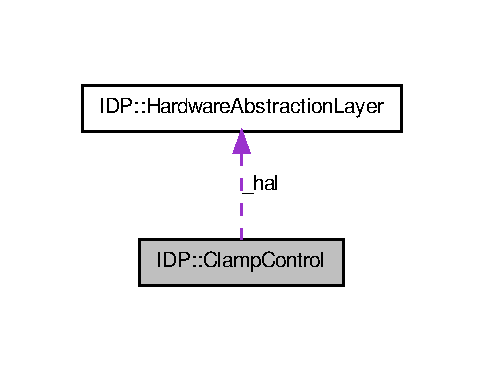
\includegraphics[width=232pt]{classIDP_1_1ClampControl__coll__graph}
\end{center}
\end{figure}
\subsection*{Public Member Functions}
\begin{DoxyCompactItemize}
\item 
\hyperlink{classIDP_1_1ClampControl_a0359cb52415c35a06521d1130e4f0795}{ClampControl} (\hyperlink{classIDP_1_1HardwareAbstractionLayer}{HardwareAbstractionLayer} $\ast$hal)
\begin{DoxyCompactList}\small\item\em Initialise the class, storing the const pointer to the HAL. \item\end{DoxyCompactList}\item 
void \hyperlink{classIDP_1_1ClampControl_a881ecc4fbc73c47594ecc675b9dbf3e1}{pick\_\-up} ()
\begin{DoxyCompactList}\small\item\em Pick up something using the clamp. \item\end{DoxyCompactList}\item 
void \hyperlink{classIDP_1_1ClampControl_a31573846d9f7c61a6133b9dd465eca25}{put\_\-down} ()
\begin{DoxyCompactList}\small\item\em Put something in the clamp down. \item\end{DoxyCompactList}\item 
\hyperlink{namespaceIDP_a6efd2cca14c0dae1c6458714ce0218df}{BobbinColour} \hyperlink{classIDP_1_1ClampControl_adcb72d77aa298264c67b42e9252f7688}{colour} () const 
\begin{DoxyCompactList}\small\item\em Check the bobbin colour. \item\end{DoxyCompactList}\item 
\hyperlink{namespaceIDP_adf12b2c1e1c228810b18c34a3c88c32d}{BobbinBadness} \hyperlink{classIDP_1_1ClampControl_ab9431b1477cb0785194ed1cfe0b8b328}{badness} () const 
\begin{DoxyCompactList}\small\item\em Check the bobbin badness. \item\end{DoxyCompactList}\end{DoxyCompactItemize}
\subsection*{Private Attributes}
\begin{DoxyCompactItemize}
\item 
\hyperlink{classIDP_1_1HardwareAbstractionLayer}{HardwareAbstractionLayer} $\ast$ \hyperlink{classIDP_1_1ClampControl_ac0c31fdbef30bc0c0d729843c8874475}{\_\-hal}
\end{DoxyCompactItemize}


\subsection{Detailed Description}
Manage the actuation of the clamp, as well as the detection and analysis of bobbins for their colour and badness. 

Definition at line 39 of file clamp\_\-control.h.



\subsection{Constructor \& Destructor Documentation}
\hypertarget{classIDP_1_1ClampControl_a0359cb52415c35a06521d1130e4f0795}{
\index{IDP::ClampControl@{IDP::ClampControl}!ClampControl@{ClampControl}}
\index{ClampControl@{ClampControl}!IDP::ClampControl@{IDP::ClampControl}}
\subsubsection[{ClampControl}]{\setlength{\rightskip}{0pt plus 5cm}IDP::ClampControl::ClampControl (
\begin{DoxyParamCaption}
\item[{{\bf HardwareAbstractionLayer} $\ast$}]{ hal}
\end{DoxyParamCaption}
)}}
\label{classIDP_1_1ClampControl_a0359cb52415c35a06521d1130e4f0795}


Initialise the class, storing the const pointer to the HAL. 


\begin{DoxyParams}{Parameters}
\item[{\em hal}]A const pointer to an instance of the HAL \end{DoxyParams}


Definition at line 39 of file clamp\_\-control.cc.



\subsection{Member Function Documentation}
\hypertarget{classIDP_1_1ClampControl_ab9431b1477cb0785194ed1cfe0b8b328}{
\index{IDP::ClampControl@{IDP::ClampControl}!badness@{badness}}
\index{badness@{badness}!IDP::ClampControl@{IDP::ClampControl}}
\subsubsection[{badness}]{\setlength{\rightskip}{0pt plus 5cm}{\bf BobbinBadness} IDP::ClampControl::badness (
\begin{DoxyParamCaption}
{}
\end{DoxyParamCaption}
) const}}
\label{classIDP_1_1ClampControl_ab9431b1477cb0785194ed1cfe0b8b328}


Check the bobbin badness. 

\begin{DoxyReturn}{Returns}
A BobbinBadness value to indicate current bobbin status 
\end{DoxyReturn}


Definition at line 75 of file clamp\_\-control.cc.

\hypertarget{classIDP_1_1ClampControl_adcb72d77aa298264c67b42e9252f7688}{
\index{IDP::ClampControl@{IDP::ClampControl}!colour@{colour}}
\index{colour@{colour}!IDP::ClampControl@{IDP::ClampControl}}
\subsubsection[{colour}]{\setlength{\rightskip}{0pt plus 5cm}{\bf BobbinColour} IDP::ClampControl::colour (
\begin{DoxyParamCaption}
{}
\end{DoxyParamCaption}
) const}}
\label{classIDP_1_1ClampControl_adcb72d77aa298264c67b42e9252f7688}


Check the bobbin colour. 

\begin{DoxyReturn}{Returns}
A BobbinColour value to indicate current bobbin colour 
\end{DoxyReturn}


Definition at line 65 of file clamp\_\-control.cc.

\hypertarget{classIDP_1_1ClampControl_a881ecc4fbc73c47594ecc675b9dbf3e1}{
\index{IDP::ClampControl@{IDP::ClampControl}!pick\_\-up@{pick\_\-up}}
\index{pick\_\-up@{pick\_\-up}!IDP::ClampControl@{IDP::ClampControl}}
\subsubsection[{pick\_\-up}]{\setlength{\rightskip}{0pt plus 5cm}void IDP::ClampControl::pick\_\-up (
\begin{DoxyParamCaption}
{}
\end{DoxyParamCaption}
)}}
\label{classIDP_1_1ClampControl_a881ecc4fbc73c47594ecc675b9dbf3e1}


Pick up something using the clamp. 



Definition at line 48 of file clamp\_\-control.cc.

\hypertarget{classIDP_1_1ClampControl_a31573846d9f7c61a6133b9dd465eca25}{
\index{IDP::ClampControl@{IDP::ClampControl}!put\_\-down@{put\_\-down}}
\index{put\_\-down@{put\_\-down}!IDP::ClampControl@{IDP::ClampControl}}
\subsubsection[{put\_\-down}]{\setlength{\rightskip}{0pt plus 5cm}void IDP::ClampControl::put\_\-down (
\begin{DoxyParamCaption}
{}
\end{DoxyParamCaption}
)}}
\label{classIDP_1_1ClampControl_a31573846d9f7c61a6133b9dd465eca25}


Put something in the clamp down. 



Definition at line 56 of file clamp\_\-control.cc.



\subsection{Member Data Documentation}
\hypertarget{classIDP_1_1ClampControl_ac0c31fdbef30bc0c0d729843c8874475}{
\index{IDP::ClampControl@{IDP::ClampControl}!\_\-hal@{\_\-hal}}
\index{\_\-hal@{\_\-hal}!IDP::ClampControl@{IDP::ClampControl}}
\subsubsection[{\_\-hal}]{\setlength{\rightskip}{0pt plus 5cm}{\bf HardwareAbstractionLayer}$\ast$ {\bf IDP::ClampControl::\_\-hal}\hspace{0.3cm}{\ttfamily  \mbox{[}private\mbox{]}}}}
\label{classIDP_1_1ClampControl_ac0c31fdbef30bc0c0d729843c8874475}


Definition at line 48 of file clamp\_\-control.h.



The documentation for this class was generated from the following files:\begin{DoxyCompactItemize}
\item 
src/libidp/\hyperlink{clamp__control_8h}{clamp\_\-control.h}\item 
src/libidp/\hyperlink{clamp__control_8cc}{clamp\_\-control.cc}\end{DoxyCompactItemize}

\hypertarget{classIDP_1_1HardwareAbstractionLayer}{
\section{IDP::HardwareAbstractionLayer Class Reference}
\label{classIDP_1_1HardwareAbstractionLayer}\index{IDP::HardwareAbstractionLayer@{IDP::HardwareAbstractionLayer}}
}


Provide a hardware agnostic interface to the required hardware functionality.  




{\ttfamily \#include $<$hal.h$>$}

\subsection*{Public Member Functions}
\begin{DoxyCompactItemize}
\item 
\hyperlink{classIDP_1_1HardwareAbstractionLayer_a424d40bbaed459f571b46dbb45bb8576}{HardwareAbstractionLayer} (const int robot)
\begin{DoxyCompactList}\small\item\em Initialise the HAL class. \item\end{DoxyCompactList}\item 
\hyperlink{classIDP_1_1HardwareAbstractionLayer_a0ddd51fb38c5fa8ecbfcd2004af2a468}{$\sim$HardwareAbstractionLayer} ()
\begin{DoxyCompactList}\small\item\em Destruct the robot link. \item\end{DoxyCompactList}\item 
void \hyperlink{classIDP_1_1HardwareAbstractionLayer_a300956b0e2e9f67e7f10baf036bf8616}{motors\_\-forward} (const unsigned short int speed)
\begin{DoxyCompactList}\small\item\em Drive both motors forwards at a given speed. \item\end{DoxyCompactList}\item 
void \hyperlink{classIDP_1_1HardwareAbstractionLayer_ac81fbf6aa2bb93837ed276c47556a398}{motors\_\-backward} (const unsigned short int speed)
\begin{DoxyCompactList}\small\item\em Drive both motors backwards at a given speed. \item\end{DoxyCompactList}\item 
void \hyperlink{classIDP_1_1HardwareAbstractionLayer_acf3d3dd4e05c4b50cb31b4d35f21abbf}{motor\_\-left\_\-forward} (const unsigned short int speed)
\begin{DoxyCompactList}\small\item\em Drive the left motor forward at the given speed. \item\end{DoxyCompactList}\item 
void \hyperlink{classIDP_1_1HardwareAbstractionLayer_aa2e2e226f2313d769e3ce226dd24d22c}{motor\_\-right\_\-forward} (const unsigned short int speed)
\begin{DoxyCompactList}\small\item\em Drive the right motor forward at the given speed. \item\end{DoxyCompactList}\item 
void \hyperlink{classIDP_1_1HardwareAbstractionLayer_a61b80e2bad5cc6a56a17350b015bfbcc}{motor\_\-left\_\-backward} (const unsigned short int speed)
\begin{DoxyCompactList}\small\item\em Drive the left motor backward at the given speed. \item\end{DoxyCompactList}\item 
void \hyperlink{classIDP_1_1HardwareAbstractionLayer_aac42c10ca431120a060f9b2c394492ae}{motor\_\-right\_\-backward} (const unsigned short int speed)
\begin{DoxyCompactList}\small\item\em Drive the right motor backward at the given speed. \item\end{DoxyCompactList}\item 
void \hyperlink{classIDP_1_1HardwareAbstractionLayer_ae38aaced2f082b6b04ebdd662349b1d2}{motors\_\-turn\_\-left} (const unsigned short int speed)
\begin{DoxyCompactList}\small\item\em Drive the motors to steer the robot to the left. \item\end{DoxyCompactList}\item 
void \hyperlink{classIDP_1_1HardwareAbstractionLayer_ad1fba0e8cb2c9ad902c8e4ec34e5e622}{motors\_\-turn\_\-right} (const unsigned short int speed)
\begin{DoxyCompactList}\small\item\em Drive the motors to steer the robot to the right. \item\end{DoxyCompactList}\item 
void \hyperlink{classIDP_1_1HardwareAbstractionLayer_a4f8f0340f3ac64c3f676b700b7e36229}{motors\_\-stop} ()
\begin{DoxyCompactList}\small\item\em Stop all motors. \item\end{DoxyCompactList}\item 
char \hyperlink{classIDP_1_1HardwareAbstractionLayer_a4867c291e34794d1bb9c0929d5514c5b}{status\_\-register} () const 
\begin{DoxyCompactList}\small\item\em Read the status register and return it. \item\end{DoxyCompactList}\item 
void \hyperlink{classIDP_1_1HardwareAbstractionLayer_a1902d9260758777966ab362e21f3be42}{clear\_\-status\_\-register} () const 
\begin{DoxyCompactList}\small\item\em Read the status register, discarding its value. \item\end{DoxyCompactList}\item 
const \hyperlink{structIDP_1_1LineSensors}{LineSensors} \hyperlink{classIDP_1_1HardwareAbstractionLayer_aca143d627de2ff9942069ad922d17ee5}{line\_\-following\_\-sensors} () const 
\begin{DoxyCompactList}\small\item\em Read the I/O port connected to the line following sensors, then return a struct with their current state. \item\end{DoxyCompactList}\item 
bool \hyperlink{classIDP_1_1HardwareAbstractionLayer_a4ce4bec948d6449e7cab3cfcd0de513f}{reset\_\-switch} () const 
\begin{DoxyCompactList}\small\item\em Read the reset switch and return its status. \item\end{DoxyCompactList}\item 
bool \hyperlink{classIDP_1_1HardwareAbstractionLayer_a82ef6744041c174edb7f8982f44685b7}{grabber\_\-switch} () const 
\begin{DoxyCompactList}\small\item\em Read the switch mounted on the grabber arm and return its status. \item\end{DoxyCompactList}\item 
unsigned short int \hyperlink{classIDP_1_1HardwareAbstractionLayer_ae4f163981d213ff3dea4b21e8aa92063}{colour\_\-ldr} () const 
\begin{DoxyCompactList}\small\item\em Get the analogue reading from the LDR used to detect colour. \item\end{DoxyCompactList}\item 
unsigned short int \hyperlink{classIDP_1_1HardwareAbstractionLayer_af4a8cb5072cf89263b97a3e8e1727da8}{bad\_\-bobbin\_\-ldr} () const 
\begin{DoxyCompactList}\small\item\em Get the analogue reading from the LDR used to detect the bad bobbin. \item\end{DoxyCompactList}\item 
void \hyperlink{classIDP_1_1HardwareAbstractionLayer_a0ffde4a54900074b646efd285d9d6807}{indication\_\-LEDs} (const bool led\_\-0, const bool led\_\-1, const bool led\_\-2)
\begin{DoxyCompactList}\small\item\em Set the bobbin colour indication LEDs. \item\end{DoxyCompactList}\item 
void \hyperlink{classIDP_1_1HardwareAbstractionLayer_a6574abe8852976bfa94c00e13d8c1686}{colour\_\-LED} (const bool status)
\begin{DoxyCompactList}\small\item\em Turn on and off the LED used to light up the bobbin for colour detection. \item\end{DoxyCompactList}\item 
void \hyperlink{classIDP_1_1HardwareAbstractionLayer_ad2feaf269fbcda10fb1192b575a4963a}{bad\_\-bobbin\_\-LED} (const bool status)
\begin{DoxyCompactList}\small\item\em Turn on and off the LED used to light up the top of the bobbin, for bad bobbin detection. \item\end{DoxyCompactList}\item 
void \hyperlink{classIDP_1_1HardwareAbstractionLayer_a44d5a4c942332ba9ffe027de3dba83f0}{grabber\_\-jaw} (const bool status)
\begin{DoxyCompactList}\small\item\em Turn the grabber jaw actuator on or off. \item\end{DoxyCompactList}\item 
void \hyperlink{classIDP_1_1HardwareAbstractionLayer_a0f036b16f1f55a257c2b552035d2a1a9}{grabber\_\-lift} (const bool status)
\begin{DoxyCompactList}\small\item\em Turn the grabber lift mechanism actuator on or off. \item\end{DoxyCompactList}\item 
void \hyperlink{classIDP_1_1HardwareAbstractionLayer_ad50b39b58566064c5bb5b0500f2d750e}{enable\_\-emergency\_\-stop} (void)
\begin{DoxyCompactList}\small\item\em Set the emergency stop registers so that the front microswitch will trigger a stop. \item\end{DoxyCompactList}\end{DoxyCompactItemize}
\subsection*{Private Member Functions}
\begin{DoxyCompactItemize}
\item 
bool \hyperlink{classIDP_1_1HardwareAbstractionLayer_a965df71af228cf82465e4e9ef6a6e1b0}{check\_\-max\_\-speed} (const unsigned short int speed) const 
\begin{DoxyCompactList}\small\item\em Check the motor speed against the set maximum, printing an error and returning true if the speed exceeds that value. \item\end{DoxyCompactList}\end{DoxyCompactItemize}
\subsection*{Private Attributes}
\begin{DoxyCompactItemize}
\item 
robot\_\-link $\ast$ \hyperlink{classIDP_1_1HardwareAbstractionLayer_a1a363a3cab8fe7fa099b19395335c0ba}{rlink}
\item 
unsigned short int \hyperlink{classIDP_1_1HardwareAbstractionLayer_a89e089becb312ef6ffe0fbc18f409b99}{\_\-port7}
\end{DoxyCompactItemize}


\subsection{Detailed Description}
Provide a hardware agnostic interface to the required hardware functionality. 

Definition at line 53 of file hal.h.



\subsection{Constructor \& Destructor Documentation}
\hypertarget{classIDP_1_1HardwareAbstractionLayer_a424d40bbaed459f571b46dbb45bb8576}{
\index{IDP::HardwareAbstractionLayer@{IDP::HardwareAbstractionLayer}!HardwareAbstractionLayer@{HardwareAbstractionLayer}}
\index{HardwareAbstractionLayer@{HardwareAbstractionLayer}!IDP::HardwareAbstractionLayer@{IDP::HardwareAbstractionLayer}}
\subsubsection[{HardwareAbstractionLayer}]{\setlength{\rightskip}{0pt plus 5cm}IDP::HardwareAbstractionLayer::HardwareAbstractionLayer (
\begin{DoxyParamCaption}
\item[{const int}]{ robot = {\ttfamily 0}}
\end{DoxyParamCaption}
)}}
\label{classIDP_1_1HardwareAbstractionLayer_a424d40bbaed459f571b46dbb45bb8576}


Initialise the HAL class. 

Establishes the link to the robot. 

Definition at line 31 of file hal.cc.

\hypertarget{classIDP_1_1HardwareAbstractionLayer_a0ddd51fb38c5fa8ecbfcd2004af2a468}{
\index{IDP::HardwareAbstractionLayer@{IDP::HardwareAbstractionLayer}!$\sim$HardwareAbstractionLayer@{$\sim$HardwareAbstractionLayer}}
\index{$\sim$HardwareAbstractionLayer@{$\sim$HardwareAbstractionLayer}!IDP::HardwareAbstractionLayer@{IDP::HardwareAbstractionLayer}}
\subsubsection[{$\sim$HardwareAbstractionLayer}]{\setlength{\rightskip}{0pt plus 5cm}IDP::HardwareAbstractionLayer::$\sim$HardwareAbstractionLayer (
\begin{DoxyParamCaption}
{}
\end{DoxyParamCaption}
)}}
\label{classIDP_1_1HardwareAbstractionLayer_a0ddd51fb38c5fa8ecbfcd2004af2a468}


Destruct the robot link. 



Definition at line 78 of file hal.cc.



\subsection{Member Function Documentation}
\hypertarget{classIDP_1_1HardwareAbstractionLayer_af4a8cb5072cf89263b97a3e8e1727da8}{
\index{IDP::HardwareAbstractionLayer@{IDP::HardwareAbstractionLayer}!bad\_\-bobbin\_\-ldr@{bad\_\-bobbin\_\-ldr}}
\index{bad\_\-bobbin\_\-ldr@{bad\_\-bobbin\_\-ldr}!IDP::HardwareAbstractionLayer@{IDP::HardwareAbstractionLayer}}
\subsubsection[{bad\_\-bobbin\_\-ldr}]{\setlength{\rightskip}{0pt plus 5cm}unsigned short int IDP::HardwareAbstractionLayer::bad\_\-bobbin\_\-ldr (
\begin{DoxyParamCaption}
{}
\end{DoxyParamCaption}
) const}}
\label{classIDP_1_1HardwareAbstractionLayer_af4a8cb5072cf89263b97a3e8e1727da8}


Get the analogue reading from the LDR used to detect the bad bobbin. 

\begin{DoxyReturn}{Returns}
The analogue reading value 
\end{DoxyReturn}


Definition at line 348 of file hal.cc.

\hypertarget{classIDP_1_1HardwareAbstractionLayer_ad2feaf269fbcda10fb1192b575a4963a}{
\index{IDP::HardwareAbstractionLayer@{IDP::HardwareAbstractionLayer}!bad\_\-bobbin\_\-LED@{bad\_\-bobbin\_\-LED}}
\index{bad\_\-bobbin\_\-LED@{bad\_\-bobbin\_\-LED}!IDP::HardwareAbstractionLayer@{IDP::HardwareAbstractionLayer}}
\subsubsection[{bad\_\-bobbin\_\-LED}]{\setlength{\rightskip}{0pt plus 5cm}void IDP::HardwareAbstractionLayer::bad\_\-bobbin\_\-LED (
\begin{DoxyParamCaption}
\item[{const bool}]{ status}
\end{DoxyParamCaption}
)}}
\label{classIDP_1_1HardwareAbstractionLayer_ad2feaf269fbcda10fb1192b575a4963a}


Turn on and off the LED used to light up the top of the bobbin, for bad bobbin detection. 


\begin{DoxyParams}{Parameters}
{\em status} & Whether the LED should be on or off (true=on) \\
\hline
\end{DoxyParams}


Definition at line 402 of file hal.cc.

\hypertarget{classIDP_1_1HardwareAbstractionLayer_a965df71af228cf82465e4e9ef6a6e1b0}{
\index{IDP::HardwareAbstractionLayer@{IDP::HardwareAbstractionLayer}!check\_\-max\_\-speed@{check\_\-max\_\-speed}}
\index{check\_\-max\_\-speed@{check\_\-max\_\-speed}!IDP::HardwareAbstractionLayer@{IDP::HardwareAbstractionLayer}}
\subsubsection[{check\_\-max\_\-speed}]{\setlength{\rightskip}{0pt plus 5cm}bool IDP::HardwareAbstractionLayer::check\_\-max\_\-speed (
\begin{DoxyParamCaption}
\item[{const unsigned short int}]{ speed}
\end{DoxyParamCaption}
) const\hspace{0.3cm}{\ttfamily  \mbox{[}private\mbox{]}}}}
\label{classIDP_1_1HardwareAbstractionLayer_a965df71af228cf82465e4e9ef6a6e1b0}


Check the motor speed against the set maximum, printing an error and returning true if the speed exceeds that value. 


\begin{DoxyParams}{Parameters}
{\em speed} & The speed to check \\
\hline
\end{DoxyParams}
\begin{DoxyReturn}{Returns}
true if the speed is too high, false if okay 
\end{DoxyReturn}


Definition at line 467 of file hal.cc.

\hypertarget{classIDP_1_1HardwareAbstractionLayer_a1902d9260758777966ab362e21f3be42}{
\index{IDP::HardwareAbstractionLayer@{IDP::HardwareAbstractionLayer}!clear\_\-status\_\-register@{clear\_\-status\_\-register}}
\index{clear\_\-status\_\-register@{clear\_\-status\_\-register}!IDP::HardwareAbstractionLayer@{IDP::HardwareAbstractionLayer}}
\subsubsection[{clear\_\-status\_\-register}]{\setlength{\rightskip}{0pt plus 5cm}void IDP::HardwareAbstractionLayer::clear\_\-status\_\-register (
\begin{DoxyParamCaption}
{}
\end{DoxyParamCaption}
) const}}
\label{classIDP_1_1HardwareAbstractionLayer_a1902d9260758777966ab362e21f3be42}


Read the status register, discarding its value. 



Definition at line 278 of file hal.cc.

\hypertarget{classIDP_1_1HardwareAbstractionLayer_ae4f163981d213ff3dea4b21e8aa92063}{
\index{IDP::HardwareAbstractionLayer@{IDP::HardwareAbstractionLayer}!colour\_\-ldr@{colour\_\-ldr}}
\index{colour\_\-ldr@{colour\_\-ldr}!IDP::HardwareAbstractionLayer@{IDP::HardwareAbstractionLayer}}
\subsubsection[{colour\_\-ldr}]{\setlength{\rightskip}{0pt plus 5cm}unsigned short int IDP::HardwareAbstractionLayer::colour\_\-ldr (
\begin{DoxyParamCaption}
{}
\end{DoxyParamCaption}
) const}}
\label{classIDP_1_1HardwareAbstractionLayer_ae4f163981d213ff3dea4b21e8aa92063}


Get the analogue reading from the LDR used to detect colour. 

\begin{DoxyReturn}{Returns}
The analogue reading value 
\end{DoxyReturn}


Definition at line 338 of file hal.cc.

\hypertarget{classIDP_1_1HardwareAbstractionLayer_a6574abe8852976bfa94c00e13d8c1686}{
\index{IDP::HardwareAbstractionLayer@{IDP::HardwareAbstractionLayer}!colour\_\-LED@{colour\_\-LED}}
\index{colour\_\-LED@{colour\_\-LED}!IDP::HardwareAbstractionLayer@{IDP::HardwareAbstractionLayer}}
\subsubsection[{colour\_\-LED}]{\setlength{\rightskip}{0pt plus 5cm}void IDP::HardwareAbstractionLayer::colour\_\-LED (
\begin{DoxyParamCaption}
\item[{const bool}]{ status}
\end{DoxyParamCaption}
)}}
\label{classIDP_1_1HardwareAbstractionLayer_a6574abe8852976bfa94c00e13d8c1686}


Turn on and off the LED used to light up the bobbin for colour detection. 


\begin{DoxyParams}{Parameters}
{\em status} & Whether the LED should be on (true) or off (false). \\
\hline
\end{DoxyParams}


Definition at line 387 of file hal.cc.

\hypertarget{classIDP_1_1HardwareAbstractionLayer_ad50b39b58566064c5bb5b0500f2d750e}{
\index{IDP::HardwareAbstractionLayer@{IDP::HardwareAbstractionLayer}!enable\_\-emergency\_\-stop@{enable\_\-emergency\_\-stop}}
\index{enable\_\-emergency\_\-stop@{enable\_\-emergency\_\-stop}!IDP::HardwareAbstractionLayer@{IDP::HardwareAbstractionLayer}}
\subsubsection[{enable\_\-emergency\_\-stop}]{\setlength{\rightskip}{0pt plus 5cm}void IDP::HardwareAbstractionLayer::enable\_\-emergency\_\-stop (
\begin{DoxyParamCaption}
\item[{void}]{}
\end{DoxyParamCaption}
)}}
\label{classIDP_1_1HardwareAbstractionLayer_ad50b39b58566064c5bb5b0500f2d750e}


Set the emergency stop registers so that the front microswitch will trigger a stop. 



Definition at line 453 of file hal.cc.

\hypertarget{classIDP_1_1HardwareAbstractionLayer_a44d5a4c942332ba9ffe027de3dba83f0}{
\index{IDP::HardwareAbstractionLayer@{IDP::HardwareAbstractionLayer}!grabber\_\-jaw@{grabber\_\-jaw}}
\index{grabber\_\-jaw@{grabber\_\-jaw}!IDP::HardwareAbstractionLayer@{IDP::HardwareAbstractionLayer}}
\subsubsection[{grabber\_\-jaw}]{\setlength{\rightskip}{0pt plus 5cm}void IDP::HardwareAbstractionLayer::grabber\_\-jaw (
\begin{DoxyParamCaption}
\item[{const bool}]{ status}
\end{DoxyParamCaption}
)}}
\label{classIDP_1_1HardwareAbstractionLayer_a44d5a4c942332ba9ffe027de3dba83f0}


Turn the grabber jaw actuator on or off. 


\begin{DoxyParams}{Parameters}
{\em status} & Jaw actuator status (true=on) \\
\hline
\end{DoxyParams}


Definition at line 417 of file hal.cc.

\hypertarget{classIDP_1_1HardwareAbstractionLayer_a0f036b16f1f55a257c2b552035d2a1a9}{
\index{IDP::HardwareAbstractionLayer@{IDP::HardwareAbstractionLayer}!grabber\_\-lift@{grabber\_\-lift}}
\index{grabber\_\-lift@{grabber\_\-lift}!IDP::HardwareAbstractionLayer@{IDP::HardwareAbstractionLayer}}
\subsubsection[{grabber\_\-lift}]{\setlength{\rightskip}{0pt plus 5cm}void IDP::HardwareAbstractionLayer::grabber\_\-lift (
\begin{DoxyParamCaption}
\item[{const bool}]{ status}
\end{DoxyParamCaption}
)}}
\label{classIDP_1_1HardwareAbstractionLayer_a0f036b16f1f55a257c2b552035d2a1a9}


Turn the grabber lift mechanism actuator on or off. 


\begin{DoxyParams}{Parameters}
{\em status} & Lift actuator status (true=on) \\
\hline
\end{DoxyParams}


Definition at line 435 of file hal.cc.

\hypertarget{classIDP_1_1HardwareAbstractionLayer_a82ef6744041c174edb7f8982f44685b7}{
\index{IDP::HardwareAbstractionLayer@{IDP::HardwareAbstractionLayer}!grabber\_\-switch@{grabber\_\-switch}}
\index{grabber\_\-switch@{grabber\_\-switch}!IDP::HardwareAbstractionLayer@{IDP::HardwareAbstractionLayer}}
\subsubsection[{grabber\_\-switch}]{\setlength{\rightskip}{0pt plus 5cm}bool IDP::HardwareAbstractionLayer::grabber\_\-switch (
\begin{DoxyParamCaption}
{}
\end{DoxyParamCaption}
) const}}
\label{classIDP_1_1HardwareAbstractionLayer_a82ef6744041c174edb7f8982f44685b7}


Read the switch mounted on the grabber arm and return its status. 

\begin{DoxyReturn}{Returns}
The current value of the switch, true if pressed 
\end{DoxyReturn}


Definition at line 319 of file hal.cc.

\hypertarget{classIDP_1_1HardwareAbstractionLayer_a0ffde4a54900074b646efd285d9d6807}{
\index{IDP::HardwareAbstractionLayer@{IDP::HardwareAbstractionLayer}!indication\_\-LEDs@{indication\_\-LEDs}}
\index{indication\_\-LEDs@{indication\_\-LEDs}!IDP::HardwareAbstractionLayer@{IDP::HardwareAbstractionLayer}}
\subsubsection[{indication\_\-LEDs}]{\setlength{\rightskip}{0pt plus 5cm}void IDP::HardwareAbstractionLayer::indication\_\-LEDs (
\begin{DoxyParamCaption}
\item[{const bool}]{ led\_\-0, }
\item[{const bool}]{ led\_\-1, }
\item[{const bool}]{ led\_\-2}
\end{DoxyParamCaption}
)}}
\label{classIDP_1_1HardwareAbstractionLayer_a0ffde4a54900074b646efd285d9d6807}


Set the bobbin colour indication LEDs. 


\begin{DoxyParams}{Parameters}
{\em led\_\-0} & Whether LED0 should be on or off (true=on) \\
\hline
{\em led\_\-1} & Whether LED1 should be on or off (true=on) \\
\hline
{\em led\_\-2} & Whether LED2 should be on or off (true=on) \\
\hline
\end{DoxyParams}


Definition at line 360 of file hal.cc.

\hypertarget{classIDP_1_1HardwareAbstractionLayer_aca143d627de2ff9942069ad922d17ee5}{
\index{IDP::HardwareAbstractionLayer@{IDP::HardwareAbstractionLayer}!line\_\-following\_\-sensors@{line\_\-following\_\-sensors}}
\index{line\_\-following\_\-sensors@{line\_\-following\_\-sensors}!IDP::HardwareAbstractionLayer@{IDP::HardwareAbstractionLayer}}
\subsubsection[{line\_\-following\_\-sensors}]{\setlength{\rightskip}{0pt plus 5cm}const {\bf LineSensors} IDP::HardwareAbstractionLayer::line\_\-following\_\-sensors (
\begin{DoxyParamCaption}
{}
\end{DoxyParamCaption}
) const}}
\label{classIDP_1_1HardwareAbstractionLayer_aca143d627de2ff9942069ad922d17ee5}


Read the I/O port connected to the line following sensors, then return a struct with their current state. 

\begin{DoxyReturn}{Returns}
A \hyperlink{structIDP_1_1LineSensors}{LineSensors} struct containing the current state of the sensors 
\end{DoxyReturn}


Definition at line 241 of file hal.cc.

\hypertarget{classIDP_1_1HardwareAbstractionLayer_a61b80e2bad5cc6a56a17350b015bfbcc}{
\index{IDP::HardwareAbstractionLayer@{IDP::HardwareAbstractionLayer}!motor\_\-left\_\-backward@{motor\_\-left\_\-backward}}
\index{motor\_\-left\_\-backward@{motor\_\-left\_\-backward}!IDP::HardwareAbstractionLayer@{IDP::HardwareAbstractionLayer}}
\subsubsection[{motor\_\-left\_\-backward}]{\setlength{\rightskip}{0pt plus 5cm}void IDP::HardwareAbstractionLayer::motor\_\-left\_\-backward (
\begin{DoxyParamCaption}
\item[{const unsigned short int}]{ speed}
\end{DoxyParamCaption}
)}}
\label{classIDP_1_1HardwareAbstractionLayer_a61b80e2bad5cc6a56a17350b015bfbcc}


Drive the left motor backward at the given speed. 


\begin{DoxyParams}{Parameters}
{\em speed} & The speed at which to drive the motor \\
\hline
\end{DoxyParams}


Definition at line 158 of file hal.cc.

\hypertarget{classIDP_1_1HardwareAbstractionLayer_acf3d3dd4e05c4b50cb31b4d35f21abbf}{
\index{IDP::HardwareAbstractionLayer@{IDP::HardwareAbstractionLayer}!motor\_\-left\_\-forward@{motor\_\-left\_\-forward}}
\index{motor\_\-left\_\-forward@{motor\_\-left\_\-forward}!IDP::HardwareAbstractionLayer@{IDP::HardwareAbstractionLayer}}
\subsubsection[{motor\_\-left\_\-forward}]{\setlength{\rightskip}{0pt plus 5cm}void IDP::HardwareAbstractionLayer::motor\_\-left\_\-forward (
\begin{DoxyParamCaption}
\item[{const unsigned short int}]{ speed}
\end{DoxyParamCaption}
)}}
\label{classIDP_1_1HardwareAbstractionLayer_acf3d3dd4e05c4b50cb31b4d35f21abbf}


Drive the left motor forward at the given speed. 


\begin{DoxyParams}{Parameters}
{\em speed} & The speed at which to drive the motor \\
\hline
\end{DoxyParams}


Definition at line 124 of file hal.cc.

\hypertarget{classIDP_1_1HardwareAbstractionLayer_aac42c10ca431120a060f9b2c394492ae}{
\index{IDP::HardwareAbstractionLayer@{IDP::HardwareAbstractionLayer}!motor\_\-right\_\-backward@{motor\_\-right\_\-backward}}
\index{motor\_\-right\_\-backward@{motor\_\-right\_\-backward}!IDP::HardwareAbstractionLayer@{IDP::HardwareAbstractionLayer}}
\subsubsection[{motor\_\-right\_\-backward}]{\setlength{\rightskip}{0pt plus 5cm}void IDP::HardwareAbstractionLayer::motor\_\-right\_\-backward (
\begin{DoxyParamCaption}
\item[{const unsigned short int}]{ speed}
\end{DoxyParamCaption}
)}}
\label{classIDP_1_1HardwareAbstractionLayer_aac42c10ca431120a060f9b2c394492ae}


Drive the right motor backward at the given speed. 


\begin{DoxyParams}{Parameters}
{\em speed} & The speed at which to drive the motor \\
\hline
\end{DoxyParams}


Definition at line 175 of file hal.cc.

\hypertarget{classIDP_1_1HardwareAbstractionLayer_aa2e2e226f2313d769e3ce226dd24d22c}{
\index{IDP::HardwareAbstractionLayer@{IDP::HardwareAbstractionLayer}!motor\_\-right\_\-forward@{motor\_\-right\_\-forward}}
\index{motor\_\-right\_\-forward@{motor\_\-right\_\-forward}!IDP::HardwareAbstractionLayer@{IDP::HardwareAbstractionLayer}}
\subsubsection[{motor\_\-right\_\-forward}]{\setlength{\rightskip}{0pt plus 5cm}void IDP::HardwareAbstractionLayer::motor\_\-right\_\-forward (
\begin{DoxyParamCaption}
\item[{const unsigned short int}]{ speed}
\end{DoxyParamCaption}
)}}
\label{classIDP_1_1HardwareAbstractionLayer_aa2e2e226f2313d769e3ce226dd24d22c}


Drive the right motor forward at the given speed. 


\begin{DoxyParams}{Parameters}
{\em speed} & The speed at which to drive the motor \\
\hline
\end{DoxyParams}


Definition at line 141 of file hal.cc.

\hypertarget{classIDP_1_1HardwareAbstractionLayer_ac81fbf6aa2bb93837ed276c47556a398}{
\index{IDP::HardwareAbstractionLayer@{IDP::HardwareAbstractionLayer}!motors\_\-backward@{motors\_\-backward}}
\index{motors\_\-backward@{motors\_\-backward}!IDP::HardwareAbstractionLayer@{IDP::HardwareAbstractionLayer}}
\subsubsection[{motors\_\-backward}]{\setlength{\rightskip}{0pt plus 5cm}void IDP::HardwareAbstractionLayer::motors\_\-backward (
\begin{DoxyParamCaption}
\item[{const unsigned short int}]{ speed}
\end{DoxyParamCaption}
)}}
\label{classIDP_1_1HardwareAbstractionLayer_ac81fbf6aa2bb93837ed276c47556a398}


Drive both motors backwards at a given speed. 


\begin{DoxyParams}{Parameters}
{\em speed} & The speed to drive at, 0 to 127 \\
\hline
\end{DoxyParams}


Definition at line 107 of file hal.cc.

\hypertarget{classIDP_1_1HardwareAbstractionLayer_a300956b0e2e9f67e7f10baf036bf8616}{
\index{IDP::HardwareAbstractionLayer@{IDP::HardwareAbstractionLayer}!motors\_\-forward@{motors\_\-forward}}
\index{motors\_\-forward@{motors\_\-forward}!IDP::HardwareAbstractionLayer@{IDP::HardwareAbstractionLayer}}
\subsubsection[{motors\_\-forward}]{\setlength{\rightskip}{0pt plus 5cm}void IDP::HardwareAbstractionLayer::motors\_\-forward (
\begin{DoxyParamCaption}
\item[{const unsigned short int}]{ speed}
\end{DoxyParamCaption}
)}}
\label{classIDP_1_1HardwareAbstractionLayer_a300956b0e2e9f67e7f10baf036bf8616}


Drive both motors forwards at a given speed. 


\begin{DoxyParams}{Parameters}
{\em speed} & The speed to drive at, 0 to 127 \\
\hline
\end{DoxyParams}


Definition at line 90 of file hal.cc.

\hypertarget{classIDP_1_1HardwareAbstractionLayer_a4f8f0340f3ac64c3f676b700b7e36229}{
\index{IDP::HardwareAbstractionLayer@{IDP::HardwareAbstractionLayer}!motors\_\-stop@{motors\_\-stop}}
\index{motors\_\-stop@{motors\_\-stop}!IDP::HardwareAbstractionLayer@{IDP::HardwareAbstractionLayer}}
\subsubsection[{motors\_\-stop}]{\setlength{\rightskip}{0pt plus 5cm}void IDP::HardwareAbstractionLayer::motors\_\-stop (
\begin{DoxyParamCaption}
{}
\end{DoxyParamCaption}
)}}
\label{classIDP_1_1HardwareAbstractionLayer_a4f8f0340f3ac64c3f676b700b7e36229}


Stop all motors. 



Definition at line 225 of file hal.cc.

\hypertarget{classIDP_1_1HardwareAbstractionLayer_ae38aaced2f082b6b04ebdd662349b1d2}{
\index{IDP::HardwareAbstractionLayer@{IDP::HardwareAbstractionLayer}!motors\_\-turn\_\-left@{motors\_\-turn\_\-left}}
\index{motors\_\-turn\_\-left@{motors\_\-turn\_\-left}!IDP::HardwareAbstractionLayer@{IDP::HardwareAbstractionLayer}}
\subsubsection[{motors\_\-turn\_\-left}]{\setlength{\rightskip}{0pt plus 5cm}void IDP::HardwareAbstractionLayer::motors\_\-turn\_\-left (
\begin{DoxyParamCaption}
\item[{const unsigned short int}]{ speed}
\end{DoxyParamCaption}
)}}
\label{classIDP_1_1HardwareAbstractionLayer_ae38aaced2f082b6b04ebdd662349b1d2}


Drive the motors to steer the robot to the left. 


\begin{DoxyParams}{Parameters}
{\em speed} & The speed to drive at, 0 to 127 \\
\hline
\end{DoxyParams}


Definition at line 192 of file hal.cc.

\hypertarget{classIDP_1_1HardwareAbstractionLayer_ad1fba0e8cb2c9ad902c8e4ec34e5e622}{
\index{IDP::HardwareAbstractionLayer@{IDP::HardwareAbstractionLayer}!motors\_\-turn\_\-right@{motors\_\-turn\_\-right}}
\index{motors\_\-turn\_\-right@{motors\_\-turn\_\-right}!IDP::HardwareAbstractionLayer@{IDP::HardwareAbstractionLayer}}
\subsubsection[{motors\_\-turn\_\-right}]{\setlength{\rightskip}{0pt plus 5cm}void IDP::HardwareAbstractionLayer::motors\_\-turn\_\-right (
\begin{DoxyParamCaption}
\item[{const unsigned short int}]{ speed}
\end{DoxyParamCaption}
)}}
\label{classIDP_1_1HardwareAbstractionLayer_ad1fba0e8cb2c9ad902c8e4ec34e5e622}


Drive the motors to steer the robot to the right. 


\begin{DoxyParams}{Parameters}
{\em speed} & The speed to drive at, 0 to 127 \\
\hline
\end{DoxyParams}


Definition at line 209 of file hal.cc.

\hypertarget{classIDP_1_1HardwareAbstractionLayer_a4ce4bec948d6449e7cab3cfcd0de513f}{
\index{IDP::HardwareAbstractionLayer@{IDP::HardwareAbstractionLayer}!reset\_\-switch@{reset\_\-switch}}
\index{reset\_\-switch@{reset\_\-switch}!IDP::HardwareAbstractionLayer@{IDP::HardwareAbstractionLayer}}
\subsubsection[{reset\_\-switch}]{\setlength{\rightskip}{0pt plus 5cm}bool IDP::HardwareAbstractionLayer::reset\_\-switch (
\begin{DoxyParamCaption}
{}
\end{DoxyParamCaption}
) const}}
\label{classIDP_1_1HardwareAbstractionLayer_a4ce4bec948d6449e7cab3cfcd0de513f}


Read the reset switch and return its status. 

\begin{DoxyReturn}{Returns}
The current value of the switch, true if pressed 
\end{DoxyReturn}


Definition at line 300 of file hal.cc.

\hypertarget{classIDP_1_1HardwareAbstractionLayer_a4867c291e34794d1bb9c0929d5514c5b}{
\index{IDP::HardwareAbstractionLayer@{IDP::HardwareAbstractionLayer}!status\_\-register@{status\_\-register}}
\index{status\_\-register@{status\_\-register}!IDP::HardwareAbstractionLayer@{IDP::HardwareAbstractionLayer}}
\subsubsection[{status\_\-register}]{\setlength{\rightskip}{0pt plus 5cm}char IDP::HardwareAbstractionLayer::status\_\-register (
\begin{DoxyParamCaption}
{}
\end{DoxyParamCaption}
) const}}
\label{classIDP_1_1HardwareAbstractionLayer_a4867c291e34794d1bb9c0929d5514c5b}


Read the status register and return it. 

\begin{DoxyReturn}{Returns}
The STATUS register 
\end{DoxyReturn}


Definition at line 289 of file hal.cc.



\subsection{Member Data Documentation}
\hypertarget{classIDP_1_1HardwareAbstractionLayer_a89e089becb312ef6ffe0fbc18f409b99}{
\index{IDP::HardwareAbstractionLayer@{IDP::HardwareAbstractionLayer}!\_\-port7@{\_\-port7}}
\index{\_\-port7@{\_\-port7}!IDP::HardwareAbstractionLayer@{IDP::HardwareAbstractionLayer}}
\subsubsection[{\_\-port7}]{\setlength{\rightskip}{0pt plus 5cm}unsigned short int {\bf IDP::HardwareAbstractionLayer::\_\-port7}\hspace{0.3cm}{\ttfamily  \mbox{[}private\mbox{]}}}}
\label{classIDP_1_1HardwareAbstractionLayer_a89e089becb312ef6ffe0fbc18f409b99}


Definition at line 84 of file hal.h.

\hypertarget{classIDP_1_1HardwareAbstractionLayer_a1a363a3cab8fe7fa099b19395335c0ba}{
\index{IDP::HardwareAbstractionLayer@{IDP::HardwareAbstractionLayer}!rlink@{rlink}}
\index{rlink@{rlink}!IDP::HardwareAbstractionLayer@{IDP::HardwareAbstractionLayer}}
\subsubsection[{rlink}]{\setlength{\rightskip}{0pt plus 5cm}robot\_\-link$\ast$ {\bf IDP::HardwareAbstractionLayer::rlink}\hspace{0.3cm}{\ttfamily  \mbox{[}private\mbox{]}}}}
\label{classIDP_1_1HardwareAbstractionLayer_a1a363a3cab8fe7fa099b19395335c0ba}


Definition at line 83 of file hal.h.



The documentation for this class was generated from the following files:\begin{DoxyCompactItemize}
\item 
src/libidp/\hyperlink{hal_8h}{hal.h}\item 
src/libidp/\hyperlink{hal_8cc}{hal.cc}\end{DoxyCompactItemize}

\hypertarget{classIDP_1_1LineFollowing}{
\section{IDP::LineFollowing Class Reference}
\label{classIDP_1_1LineFollowing}\index{IDP::LineFollowing@{IDP::LineFollowing}}
}


Maintain the robot position correctly with respect to the white line markers, during driving and manouvering.  




{\ttfamily \#include $<$line\_\-following.h$>$}



Collaboration diagram for IDP::LineFollowing:\nopagebreak
\begin{figure}[H]
\begin{center}
\leavevmode
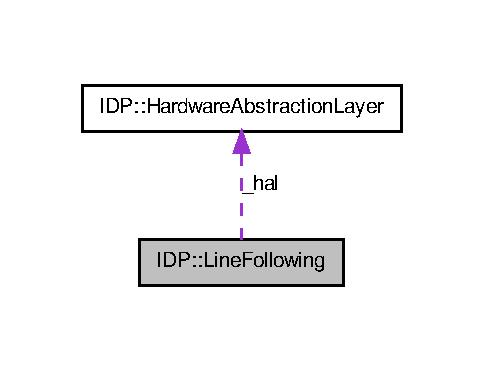
\includegraphics[width=232pt]{classIDP_1_1LineFollowing__coll__graph}
\end{center}
\end{figure}
\subsection*{Public Member Functions}
\begin{DoxyCompactItemize}
\item 
\hyperlink{classIDP_1_1LineFollowing_ab30cde971719545d81ce253ae995cc4d}{LineFollowing} (const \hyperlink{classIDP_1_1HardwareAbstractionLayer}{HardwareAbstractionLayer} $\ast$hal)
\begin{DoxyCompactList}\small\item\em Construct the Line Follower. \item\end{DoxyCompactList}\item 
void \hyperlink{classIDP_1_1LineFollowing_af578916c93854c701fccbdaef783997b}{correct\_\-steering} (int error)
\begin{DoxyCompactList}\small\item\em Correct the steering of the robot. \item\end{DoxyCompactList}\item 
void \hyperlink{classIDP_1_1LineFollowing_a35c80e04729e98dfa927159610605649}{follow\_\-line} ()
\begin{DoxyCompactList}\small\item\em Follow a line forwards, stopping when a junction is reached. \item\end{DoxyCompactList}\end{DoxyCompactItemize}


\subsection{Detailed Description}
Maintain the robot position correctly with respect to the white line markers, during driving and manouvering. 

\subsection{Constructor \& Destructor Documentation}
\hypertarget{classIDP_1_1LineFollowing_ab30cde971719545d81ce253ae995cc4d}{
\index{IDP::LineFollowing@{IDP::LineFollowing}!LineFollowing@{LineFollowing}}
\index{LineFollowing@{LineFollowing}!IDP::LineFollowing@{IDP::LineFollowing}}
\subsubsection[{LineFollowing}]{\setlength{\rightskip}{0pt plus 5cm}IDP::LineFollowing::LineFollowing (
\begin{DoxyParamCaption}
\item[{const {\bf HardwareAbstractionLayer} $\ast$}]{ hal}
\end{DoxyParamCaption}
)}}
\label{classIDP_1_1LineFollowing_ab30cde971719545d81ce253ae995cc4d}


Construct the Line Follower. 



\subsection{Member Function Documentation}
\hypertarget{classIDP_1_1LineFollowing_af578916c93854c701fccbdaef783997b}{
\index{IDP::LineFollowing@{IDP::LineFollowing}!correct\_\-steering@{correct\_\-steering}}
\index{correct\_\-steering@{correct\_\-steering}!IDP::LineFollowing@{IDP::LineFollowing}}
\subsubsection[{correct\_\-steering}]{\setlength{\rightskip}{0pt plus 5cm}void IDP::LineFollowing::correct\_\-steering (
\begin{DoxyParamCaption}
\item[{int}]{ \_\-error}
\end{DoxyParamCaption}
)}}
\label{classIDP_1_1LineFollowing_af578916c93854c701fccbdaef783997b}


Correct the steering of the robot. 


\begin{DoxyParams}{Parameters}
\item[{\em \_\-error}]A signed integer where negative is too far left, and positive is too far right \end{DoxyParams}
\hypertarget{classIDP_1_1LineFollowing_a35c80e04729e98dfa927159610605649}{
\index{IDP::LineFollowing@{IDP::LineFollowing}!follow\_\-line@{follow\_\-line}}
\index{follow\_\-line@{follow\_\-line}!IDP::LineFollowing@{IDP::LineFollowing}}
\subsubsection[{follow\_\-line}]{\setlength{\rightskip}{0pt plus 5cm}void IDP::LineFollowing::follow\_\-line (
\begin{DoxyParamCaption}
{}
\end{DoxyParamCaption}
)}}
\label{classIDP_1_1LineFollowing_a35c80e04729e98dfa927159610605649}


Follow a line forwards, stopping when a junction is reached. 



The documentation for this class was generated from the following files:\begin{DoxyCompactItemize}
\item 
libidp/\hyperlink{line__following_8h}{line\_\-following.h}\item 
libidp/\hyperlink{line__following_8cc}{line\_\-following.cc}\end{DoxyCompactItemize}

\hypertarget{structIDP_1_1LineSensors}{
\section{IDP::LineSensors Struct Reference}
\label{structIDP_1_1LineSensors}\index{IDP::LineSensors@{IDP::LineSensors}}
}


Contains the LINE or NO\_\-LINE status of each of the four IR sensors used for line following.  




{\ttfamily \#include $<$hal.h$>$}

\subsection*{Public Attributes}
\begin{DoxyCompactItemize}
\item 
\hyperlink{namespaceIDP_afc3b1d4cbb313bfc854f49d6f23b25f7}{LineSensorStatus} \hyperlink{structIDP_1_1LineSensors_a009bf6abf88cf3c732545da20148ba5e}{outer\_\-left}
\item 
\hyperlink{namespaceIDP_afc3b1d4cbb313bfc854f49d6f23b25f7}{LineSensorStatus} \hyperlink{structIDP_1_1LineSensors_ab986b625016c2f99536299b6d0af3f29}{line\_\-left}
\item 
\hyperlink{namespaceIDP_afc3b1d4cbb313bfc854f49d6f23b25f7}{LineSensorStatus} \hyperlink{structIDP_1_1LineSensors_a03e1692ac462e2e6744c9d5a7656c6f1}{line\_\-right}
\item 
\hyperlink{namespaceIDP_afc3b1d4cbb313bfc854f49d6f23b25f7}{LineSensorStatus} \hyperlink{structIDP_1_1LineSensors_afa87dc008f415429d15e35a49d52083c}{outer\_\-right}
\end{DoxyCompactItemize}


\subsection{Detailed Description}
Contains the LINE or NO\_\-LINE status of each of the four IR sensors used for line following. 

\subsection{Member Data Documentation}
\hypertarget{structIDP_1_1LineSensors_ab986b625016c2f99536299b6d0af3f29}{
\index{IDP::LineSensors@{IDP::LineSensors}!line\_\-left@{line\_\-left}}
\index{line\_\-left@{line\_\-left}!IDP::LineSensors@{IDP::LineSensors}}
\subsubsection[{line\_\-left}]{\setlength{\rightskip}{0pt plus 5cm}{\bf LineSensorStatus} {\bf IDP::LineSensors::line\_\-left}}}
\label{structIDP_1_1LineSensors_ab986b625016c2f99536299b6d0af3f29}
\hypertarget{structIDP_1_1LineSensors_a03e1692ac462e2e6744c9d5a7656c6f1}{
\index{IDP::LineSensors@{IDP::LineSensors}!line\_\-right@{line\_\-right}}
\index{line\_\-right@{line\_\-right}!IDP::LineSensors@{IDP::LineSensors}}
\subsubsection[{line\_\-right}]{\setlength{\rightskip}{0pt plus 5cm}{\bf LineSensorStatus} {\bf IDP::LineSensors::line\_\-right}}}
\label{structIDP_1_1LineSensors_a03e1692ac462e2e6744c9d5a7656c6f1}
\hypertarget{structIDP_1_1LineSensors_a009bf6abf88cf3c732545da20148ba5e}{
\index{IDP::LineSensors@{IDP::LineSensors}!outer\_\-left@{outer\_\-left}}
\index{outer\_\-left@{outer\_\-left}!IDP::LineSensors@{IDP::LineSensors}}
\subsubsection[{outer\_\-left}]{\setlength{\rightskip}{0pt plus 5cm}{\bf LineSensorStatus} {\bf IDP::LineSensors::outer\_\-left}}}
\label{structIDP_1_1LineSensors_a009bf6abf88cf3c732545da20148ba5e}
\hypertarget{structIDP_1_1LineSensors_afa87dc008f415429d15e35a49d52083c}{
\index{IDP::LineSensors@{IDP::LineSensors}!outer\_\-right@{outer\_\-right}}
\index{outer\_\-right@{outer\_\-right}!IDP::LineSensors@{IDP::LineSensors}}
\subsubsection[{outer\_\-right}]{\setlength{\rightskip}{0pt plus 5cm}{\bf LineSensorStatus} {\bf IDP::LineSensors::outer\_\-right}}}
\label{structIDP_1_1LineSensors_afa87dc008f415429d15e35a49d52083c}


The documentation for this struct was generated from the following file:\begin{DoxyCompactItemize}
\item 
libidp/\hyperlink{hal_8h}{hal.h}\end{DoxyCompactItemize}

\hypertarget{classIDP_1_1MissionSupervisor}{
\section{IDP::MissionSupervisor Class Reference}
\label{classIDP_1_1MissionSupervisor}\index{IDP::MissionSupervisor@{IDP::MissionSupervisor}}
}


{\ttfamily \#include $<$mission\_\-supervisor.h$>$}



Collaboration diagram for IDP::MissionSupervisor:
\subsection*{Public Member Functions}
\begin{DoxyCompactItemize}
\item 
\hyperlink{classIDP_1_1MissionSupervisor_afc6a54e04718d919b2b48458a47304b2}{MissionSupervisor} (int robot)
\item 
void \hyperlink{classIDP_1_1MissionSupervisor_af8c6a3073190a4479211753fe5f50a36}{drive\_\-forward} ()
\item 
void \hyperlink{classIDP_1_1MissionSupervisor_ae5d6e9a37417126da780583349b48d44}{drive\_\-backward} ()
\item 
void \hyperlink{classIDP_1_1MissionSupervisor_ad11e444b6be1d51c3339bd6397d45fd4}{stop} ()
\item 
void \hyperlink{classIDP_1_1MissionSupervisor_af147b0bec9464bb7e956a40a7f3d0fda}{test\_\-line\_\-sensor} ()
\item 
void \hyperlink{classIDP_1_1MissionSupervisor_a21be0b52e2f13c7fb373c90dae77ba23}{test\_\-line\_\-following} ()
\item 
const \hyperlink{classIDP_1_1HardwareAbstractionLayer}{HardwareAbstractionLayer} $\ast$ \hyperlink{classIDP_1_1MissionSupervisor_ae19d0c2123fda158cc45e649128fbc09}{hal} () const 
\end{DoxyCompactItemize}


\subsection{Constructor \& Destructor Documentation}
\hypertarget{classIDP_1_1MissionSupervisor_afc6a54e04718d919b2b48458a47304b2}{
\index{IDP::MissionSupervisor@{IDP::MissionSupervisor}!MissionSupervisor@{MissionSupervisor}}
\index{MissionSupervisor@{MissionSupervisor}!IDP::MissionSupervisor@{IDP::MissionSupervisor}}
\subsubsection[{MissionSupervisor}]{\setlength{\rightskip}{0pt plus 5cm}IDP::MissionSupervisor::MissionSupervisor (
\begin{DoxyParamCaption}
\item[{int}]{ robot = {\ttfamily 0}}
\end{DoxyParamCaption}
)}}
\label{classIDP_1_1MissionSupervisor_afc6a54e04718d919b2b48458a47304b2}
Construct the \hyperlink{classIDP_1_1MissionSupervisor}{MissionSupervisor}. Initialises a link to the specified robot number, or 0 if running embedded. 
\begin{DoxyParams}{Parameters}
{\em robot} & Which robot to link to, or 0 if embedded \\
\hline
\end{DoxyParams}


\subsection{Member Function Documentation}
\hypertarget{classIDP_1_1MissionSupervisor_ae5d6e9a37417126da780583349b48d44}{
\index{IDP::MissionSupervisor@{IDP::MissionSupervisor}!drive\_\-backward@{drive\_\-backward}}
\index{drive\_\-backward@{drive\_\-backward}!IDP::MissionSupervisor@{IDP::MissionSupervisor}}
\subsubsection[{drive\_\-backward}]{\setlength{\rightskip}{0pt plus 5cm}void IDP::MissionSupervisor::drive\_\-backward (
\begin{DoxyParamCaption}
{}
\end{DoxyParamCaption}
)}}
\label{classIDP_1_1MissionSupervisor_ae5d6e9a37417126da780583349b48d44}
Set both motors driving backwards. \hypertarget{classIDP_1_1MissionSupervisor_af8c6a3073190a4479211753fe5f50a36}{
\index{IDP::MissionSupervisor@{IDP::MissionSupervisor}!drive\_\-forward@{drive\_\-forward}}
\index{drive\_\-forward@{drive\_\-forward}!IDP::MissionSupervisor@{IDP::MissionSupervisor}}
\subsubsection[{drive\_\-forward}]{\setlength{\rightskip}{0pt plus 5cm}void IDP::MissionSupervisor::drive\_\-forward (
\begin{DoxyParamCaption}
{}
\end{DoxyParamCaption}
)}}
\label{classIDP_1_1MissionSupervisor_af8c6a3073190a4479211753fe5f50a36}
Set both motors driving forwards. \hypertarget{classIDP_1_1MissionSupervisor_ae19d0c2123fda158cc45e649128fbc09}{
\index{IDP::MissionSupervisor@{IDP::MissionSupervisor}!hal@{hal}}
\index{hal@{hal}!IDP::MissionSupervisor@{IDP::MissionSupervisor}}
\subsubsection[{hal}]{\setlength{\rightskip}{0pt plus 5cm}const {\bf HardwareAbstractionLayer} $\ast$ IDP::MissionSupervisor::hal (
\begin{DoxyParamCaption}
{}
\end{DoxyParamCaption}
) const}}
\label{classIDP_1_1MissionSupervisor_ae19d0c2123fda158cc45e649128fbc09}
Const accessor for the HAL \hypertarget{classIDP_1_1MissionSupervisor_ad11e444b6be1d51c3339bd6397d45fd4}{
\index{IDP::MissionSupervisor@{IDP::MissionSupervisor}!stop@{stop}}
\index{stop@{stop}!IDP::MissionSupervisor@{IDP::MissionSupervisor}}
\subsubsection[{stop}]{\setlength{\rightskip}{0pt plus 5cm}void IDP::MissionSupervisor::stop (
\begin{DoxyParamCaption}
{}
\end{DoxyParamCaption}
)}}
\label{classIDP_1_1MissionSupervisor_ad11e444b6be1d51c3339bd6397d45fd4}
Stop all motors. \hypertarget{classIDP_1_1MissionSupervisor_a21be0b52e2f13c7fb373c90dae77ba23}{
\index{IDP::MissionSupervisor@{IDP::MissionSupervisor}!test\_\-line\_\-following@{test\_\-line\_\-following}}
\index{test\_\-line\_\-following@{test\_\-line\_\-following}!IDP::MissionSupervisor@{IDP::MissionSupervisor}}
\subsubsection[{test\_\-line\_\-following}]{\setlength{\rightskip}{0pt plus 5cm}void IDP::MissionSupervisor::test\_\-line\_\-following (
\begin{DoxyParamCaption}
{}
\end{DoxyParamCaption}
)}}
\label{classIDP_1_1MissionSupervisor_a21be0b52e2f13c7fb373c90dae77ba23}
Test line following on a straight line \hypertarget{classIDP_1_1MissionSupervisor_af147b0bec9464bb7e956a40a7f3d0fda}{
\index{IDP::MissionSupervisor@{IDP::MissionSupervisor}!test\_\-line\_\-sensor@{test\_\-line\_\-sensor}}
\index{test\_\-line\_\-sensor@{test\_\-line\_\-sensor}!IDP::MissionSupervisor@{IDP::MissionSupervisor}}
\subsubsection[{test\_\-line\_\-sensor}]{\setlength{\rightskip}{0pt plus 5cm}void IDP::MissionSupervisor::test\_\-line\_\-sensor (
\begin{DoxyParamCaption}
{}
\end{DoxyParamCaption}
)}}
\label{classIDP_1_1MissionSupervisor_af147b0bec9464bb7e956a40a7f3d0fda}
Attempt to read the line sensor status 

The documentation for this class was generated from the following files:\begin{DoxyCompactItemize}
\item 
libidp/\hyperlink{mission__supervisor_8h}{mission\_\-supervisor.h}\item 
libidp/\hyperlink{mission__supervisor_8cc}{mission\_\-supervisor.cc}\end{DoxyCompactItemize}

\hypertarget{classIDP_1_1Navigation}{
\section{IDP::Navigation Class Reference}
\label{classIDP_1_1Navigation}\index{IDP::Navigation@{IDP::Navigation}}
}


{\ttfamily \#include $<$navigation.h$>$}

\subsection*{Public Member Functions}
\begin{DoxyCompactItemize}
\item 
\hyperlink{classIDP_1_1Navigation_a028ddc27093e3d5de2dfac886c15d478}{Navigation} (const \hyperlink{classIDP_1_1HardwareAbstractionLayer}{HardwareAbstractionLayer} $\ast$hal)
\item 
const \hyperlink{namespaceIDP_a1a96e566e4d675fdf20780cc96d92283}{NavigationStatus} \hyperlink{classIDP_1_1Navigation_ab5cf30dd7a21c90d2ae58309ce0ddfa6}{go} (const \hyperlink{namespaceIDP_ab9c412f0fd539b5d70385066c30465a0}{NavigationLocation} location)
\end{DoxyCompactItemize}


\subsection{Constructor \& Destructor Documentation}
\hypertarget{classIDP_1_1Navigation_a028ddc27093e3d5de2dfac886c15d478}{
\index{IDP::Navigation@{IDP::Navigation}!Navigation@{Navigation}}
\index{Navigation@{Navigation}!IDP::Navigation@{IDP::Navigation}}
\subsubsection[{Navigation}]{\setlength{\rightskip}{0pt plus 5cm}IDP::Navigation::Navigation (
\begin{DoxyParamCaption}
\item[{const {\bf HardwareAbstractionLayer} $\ast$}]{ hal}
\end{DoxyParamCaption}
)}}
\label{classIDP_1_1Navigation_a028ddc27093e3d5de2dfac886c15d478}
Initialise the class, storing the const pointer to the HAL. 
\begin{DoxyParams}{Parameters}
{\em hal} & A const pointer to an instance of the HAL \\
\hline
\end{DoxyParams}


\subsection{Member Function Documentation}
\hypertarget{classIDP_1_1Navigation_ab5cf30dd7a21c90d2ae58309ce0ddfa6}{
\index{IDP::Navigation@{IDP::Navigation}!go@{go}}
\index{go@{go}!IDP::Navigation@{IDP::Navigation}}
\subsubsection[{go}]{\setlength{\rightskip}{0pt plus 5cm}const {\bf NavigationStatus} IDP::Navigation::go (
\begin{DoxyParamCaption}
\item[{const {\bf NavigationLocation}}]{ location}
\end{DoxyParamCaption}
)}}
\label{classIDP_1_1Navigation_ab5cf30dd7a21c90d2ae58309ce0ddfa6}
Go to a location. \begin{DoxyReturn}{Returns}
A navigation status code 
\end{DoxyReturn}


The documentation for this class was generated from the following files:\begin{DoxyCompactItemize}
\item 
libidp/\hyperlink{navigation_8h}{navigation.h}\item 
libidp/\hyperlink{navigation_8cc}{navigation.cc}\end{DoxyCompactItemize}

\hypertarget{classIDP_1_1SelfTests}{
\section{IDP::SelfTests Class Reference}
\label{classIDP_1_1SelfTests}\index{IDP::SelfTests@{IDP::SelfTests}}
}


Execute a variety of functionality self tests.  




{\ttfamily \#include $<$self\_\-tests.h$>$}



Collaboration diagram for IDP::SelfTests:\nopagebreak
\begin{figure}[H]
\begin{center}
\leavevmode
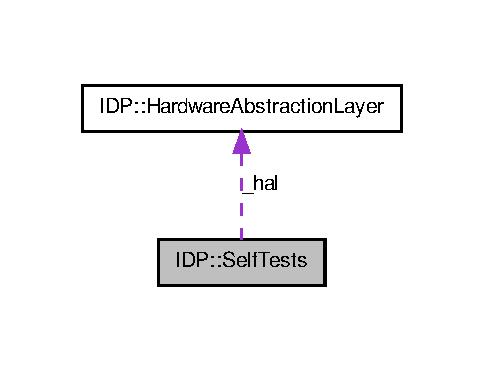
\includegraphics[width=232pt]{classIDP_1_1SelfTests__coll__graph}
\end{center}
\end{figure}
\subsection*{Public Member Functions}
\begin{DoxyCompactItemize}
\item 
\hyperlink{classIDP_1_1SelfTests_a6864b03502cc5d1ac3728b456b04238f}{SelfTests} (int robot)
\begin{DoxyCompactList}\small\item\em Constuct a \hyperlink{classIDP_1_1SelfTests}{SelfTests} instance Completely seperate to mission supervisor and initialises own link to robot, with its own HAL instance. \item\end{DoxyCompactList}\item 
\hyperlink{classIDP_1_1SelfTests_a5a49e246d28af6332dd46f8b22dcddc7}{$\sim$SelfTests} ()
\begin{DoxyCompactList}\small\item\em Destruct the \hyperlink{classIDP_1_1SelfTests}{SelfTests}, deleting the HAL. \item\end{DoxyCompactList}\item 
void \hyperlink{classIDP_1_1SelfTests_a4ff456e74d55e13599cf64db76bd2ed4}{drive\_\-forward} (void)
\begin{DoxyCompactList}\small\item\em Drive the robot forwards for a moment. \item\end{DoxyCompactList}\item 
void \hyperlink{classIDP_1_1SelfTests_a38ddef7ecdf9b7dfa69d689c9c1ac8ca}{drive\_\-backward} (void)
\begin{DoxyCompactList}\small\item\em Drive the robot backwards for a moment. \item\end{DoxyCompactList}\item 
void \hyperlink{classIDP_1_1SelfTests_a33adf462d8c408b1c7b4858e9a4ff000}{stop} (void)
\begin{DoxyCompactList}\small\item\em Stop all of the robot's motors. \item\end{DoxyCompactList}\item 
void \hyperlink{classIDP_1_1SelfTests_a3ba14e5a1ed52ff112bc742b94f06d61}{turn\_\-left} (void)
\begin{DoxyCompactList}\small\item\em Drive motors in opposite directions to turn the robot left on the spot. \item\end{DoxyCompactList}\item 
void \hyperlink{classIDP_1_1SelfTests_a4e4b66ddff2de3444f1e9383dcf463a6}{turn\_\-right} (void)
\begin{DoxyCompactList}\small\item\em Drive motors in opposite directions to turn the robot right on the spot. \item\end{DoxyCompactList}\item 
void \hyperlink{classIDP_1_1SelfTests_ae54bd0e6c01c5d1d794363cc676dbb92}{steer\_\-left} (void)
\begin{DoxyCompactList}\small\item\em Drive forwards for a moment whilst reducing the speed of the left motor relative to the right to steer left. \item\end{DoxyCompactList}\item 
void \hyperlink{classIDP_1_1SelfTests_a7f9c5999de2e7c4f59c8c5a60965e876}{steer\_\-right} (void)
\begin{DoxyCompactList}\small\item\em Drive forwards for a moment whilst reducing the speed of the right motor relative to the left to steer right. \item\end{DoxyCompactList}\item 
void \hyperlink{classIDP_1_1SelfTests_aa73ad4de6c1d2b725ed796c10f54ab7c}{line\_\-sensors} (void)
\begin{DoxyCompactList}\small\item\em Display the status (LINE or NO\_\-LINE) of each of the four IR line following sensors. \item\end{DoxyCompactList}\item 
void \hyperlink{classIDP_1_1SelfTests_a6b2e4d0517de4b73c63f1b1a475b602f}{microswitches} (void)
\begin{DoxyCompactList}\small\item\em Display the state of each of the two microswitches. \item\end{DoxyCompactList}\item 
void \hyperlink{classIDP_1_1SelfTests_a56952650637691f869ef21f7d43f1226}{LDRs} (void)
\begin{DoxyCompactList}\small\item\em Display the current ADC read from the light dependent resistor. \item\end{DoxyCompactList}\item 
void \hyperlink{classIDP_1_1SelfTests_a0ca765ac144fafaab502f4326a480486}{actuators} (void)
\begin{DoxyCompactList}\small\item\em Fire each of the actuators in turn. \item\end{DoxyCompactList}\item 
void \hyperlink{classIDP_1_1SelfTests_a0a1a40b56fee5249def567bebdb05dc1}{line\_\-following} (void)
\begin{DoxyCompactList}\small\item\em Follow a line until a junction. \item\end{DoxyCompactList}\item 
void \hyperlink{classIDP_1_1SelfTests_a896204355ca039660a12e8131578b6c3}{clamp\_\-control} (void)
\begin{DoxyCompactList}\small\item\em Use the actuators to pick up an object before placing it back down again. \item\end{DoxyCompactList}\item 
void \hyperlink{classIDP_1_1SelfTests_a66f0a3bad277e36b963b2bf3cd5df9dd}{bobbin\_\-analyse} (void)
\begin{DoxyCompactList}\small\item\em Analyse the colour of the bobbin that is currently being held in the clamp. \item\end{DoxyCompactList}\item 
void \hyperlink{classIDP_1_1SelfTests_a710347081427c05706f92bdd12f62fbe}{navigate} (void)
\begin{DoxyCompactList}\small\item\em Select a source and destination and then navigate to the destination assuming we are starting at the source. \item\end{DoxyCompactList}\item 
void \hyperlink{classIDP_1_1SelfTests_ada3dfe991573fc6b0922cace927fc4e0}{position} (void)
\begin{DoxyCompactList}\small\item\em Drive slowly looking for an object in range for pickup, then position self ready to clamp said object. \item\end{DoxyCompactList}\item 
void \hyperlink{classIDP_1_1SelfTests_abbe6e3e29b00f760e0b65f2aeb772fb5}{status\_\-LEDs} (void)
\begin{DoxyCompactList}\small\item\em Turn on each of the status LEDs (used for indicating bobbin colour) in turn. \item\end{DoxyCompactList}\item 
void \hyperlink{classIDP_1_1SelfTests_a1380b0222eef47f6d50e7cf334e4c9e7}{colour\_\-sensor\_\-LEDs} (void)
\begin{DoxyCompactList}\small\item\em Turn on each of the coloured LEDs used for colour detection in turn. \item\end{DoxyCompactList}\item 
void \hyperlink{classIDP_1_1SelfTests_aee90c71e9e93398f06dc1ad67002d7bf}{badness\_\-LED} (void)
\begin{DoxyCompactList}\small\item\em Turn on the LED used for detecting bad bobbins. \item\end{DoxyCompactList}\end{DoxyCompactItemize}
\subsection*{Private Attributes}
\begin{DoxyCompactItemize}
\item 
int \hyperlink{classIDP_1_1SelfTests_a90c60ce647f723e9a37339aadba4770c}{\_\-robot}
\item 
\hyperlink{classIDP_1_1HardwareAbstractionLayer}{HardwareAbstractionLayer} $\ast$ \hyperlink{classIDP_1_1SelfTests_a1f8a6f6c2ff26182311c8a7766db6f5a}{\_\-hal}
\end{DoxyCompactItemize}


\subsection{Detailed Description}
Execute a variety of functionality self tests. 

Definition at line 23 of file self\_\-tests.h.



\subsection{Constructor \& Destructor Documentation}
\hypertarget{classIDP_1_1SelfTests_a6864b03502cc5d1ac3728b456b04238f}{
\index{IDP::SelfTests@{IDP::SelfTests}!SelfTests@{SelfTests}}
\index{SelfTests@{SelfTests}!IDP::SelfTests@{IDP::SelfTests}}
\subsubsection[{SelfTests}]{\setlength{\rightskip}{0pt plus 5cm}IDP::SelfTests::SelfTests (
\begin{DoxyParamCaption}
\item[{int}]{ robot = {\ttfamily 0}}
\end{DoxyParamCaption}
)}}
\label{classIDP_1_1SelfTests_a6864b03502cc5d1ac3728b456b04238f}


Constuct a \hyperlink{classIDP_1_1SelfTests}{SelfTests} instance Completely seperate to mission supervisor and initialises own link to robot, with its own HAL instance. 


\begin{DoxyParams}{Parameters}
\item[{\em robot}]Which robot to link to, or 0 if embedded \end{DoxyParams}


Definition at line 29 of file self\_\-tests.cc.

\hypertarget{classIDP_1_1SelfTests_a5a49e246d28af6332dd46f8b22dcddc7}{
\index{IDP::SelfTests@{IDP::SelfTests}!$\sim$SelfTests@{$\sim$SelfTests}}
\index{$\sim$SelfTests@{$\sim$SelfTests}!IDP::SelfTests@{IDP::SelfTests}}
\subsubsection[{$\sim$SelfTests}]{\setlength{\rightskip}{0pt plus 5cm}IDP::SelfTests::$\sim$SelfTests (
\begin{DoxyParamCaption}
{}
\end{DoxyParamCaption}
)}}
\label{classIDP_1_1SelfTests_a5a49e246d28af6332dd46f8b22dcddc7}


Destruct the \hyperlink{classIDP_1_1SelfTests}{SelfTests}, deleting the HAL. 



Definition at line 39 of file self\_\-tests.cc.



\subsection{Member Function Documentation}
\hypertarget{classIDP_1_1SelfTests_a0ca765ac144fafaab502f4326a480486}{
\index{IDP::SelfTests@{IDP::SelfTests}!actuators@{actuators}}
\index{actuators@{actuators}!IDP::SelfTests@{IDP::SelfTests}}
\subsubsection[{actuators}]{\setlength{\rightskip}{0pt plus 5cm}void IDP::SelfTests::actuators (
\begin{DoxyParamCaption}
\item[{void}]{}
\end{DoxyParamCaption}
)}}
\label{classIDP_1_1SelfTests_a0ca765ac144fafaab502f4326a480486}


Fire each of the actuators in turn. 



Definition at line 177 of file self\_\-tests.cc.

\hypertarget{classIDP_1_1SelfTests_aee90c71e9e93398f06dc1ad67002d7bf}{
\index{IDP::SelfTests@{IDP::SelfTests}!badness\_\-LED@{badness\_\-LED}}
\index{badness\_\-LED@{badness\_\-LED}!IDP::SelfTests@{IDP::SelfTests}}
\subsubsection[{badness\_\-LED}]{\setlength{\rightskip}{0pt plus 5cm}void IDP::SelfTests::badness\_\-LED (
\begin{DoxyParamCaption}
\item[{void}]{}
\end{DoxyParamCaption}
)}}
\label{classIDP_1_1SelfTests_aee90c71e9e93398f06dc1ad67002d7bf}


Turn on the LED used for detecting bad bobbins. 



Definition at line 285 of file self\_\-tests.cc.

\hypertarget{classIDP_1_1SelfTests_a66f0a3bad277e36b963b2bf3cd5df9dd}{
\index{IDP::SelfTests@{IDP::SelfTests}!bobbin\_\-analyse@{bobbin\_\-analyse}}
\index{bobbin\_\-analyse@{bobbin\_\-analyse}!IDP::SelfTests@{IDP::SelfTests}}
\subsubsection[{bobbin\_\-analyse}]{\setlength{\rightskip}{0pt plus 5cm}void IDP::SelfTests::bobbin\_\-analyse (
\begin{DoxyParamCaption}
\item[{void}]{}
\end{DoxyParamCaption}
)}}
\label{classIDP_1_1SelfTests_a66f0a3bad277e36b963b2bf3cd5df9dd}


Analyse the colour of the bobbin that is currently being held in the clamp. 



Definition at line 214 of file self\_\-tests.cc.

\hypertarget{classIDP_1_1SelfTests_a896204355ca039660a12e8131578b6c3}{
\index{IDP::SelfTests@{IDP::SelfTests}!clamp\_\-control@{clamp\_\-control}}
\index{clamp\_\-control@{clamp\_\-control}!IDP::SelfTests@{IDP::SelfTests}}
\subsubsection[{clamp\_\-control}]{\setlength{\rightskip}{0pt plus 5cm}void IDP::SelfTests::clamp\_\-control (
\begin{DoxyParamCaption}
\item[{void}]{}
\end{DoxyParamCaption}
)}}
\label{classIDP_1_1SelfTests_a896204355ca039660a12e8131578b6c3}


Use the actuators to pick up an object before placing it back down again. 



Definition at line 205 of file self\_\-tests.cc.

\hypertarget{classIDP_1_1SelfTests_a1380b0222eef47f6d50e7cf334e4c9e7}{
\index{IDP::SelfTests@{IDP::SelfTests}!colour\_\-sensor\_\-LEDs@{colour\_\-sensor\_\-LEDs}}
\index{colour\_\-sensor\_\-LEDs@{colour\_\-sensor\_\-LEDs}!IDP::SelfTests@{IDP::SelfTests}}
\subsubsection[{colour\_\-sensor\_\-LEDs}]{\setlength{\rightskip}{0pt plus 5cm}void IDP::SelfTests::colour\_\-sensor\_\-LEDs (
\begin{DoxyParamCaption}
\item[{void}]{}
\end{DoxyParamCaption}
)}}
\label{classIDP_1_1SelfTests_a1380b0222eef47f6d50e7cf334e4c9e7}


Turn on each of the coloured LEDs used for colour detection in turn. 



Definition at line 277 of file self\_\-tests.cc.

\hypertarget{classIDP_1_1SelfTests_a38ddef7ecdf9b7dfa69d689c9c1ac8ca}{
\index{IDP::SelfTests@{IDP::SelfTests}!drive\_\-backward@{drive\_\-backward}}
\index{drive\_\-backward@{drive\_\-backward}!IDP::SelfTests@{IDP::SelfTests}}
\subsubsection[{drive\_\-backward}]{\setlength{\rightskip}{0pt plus 5cm}void IDP::SelfTests::drive\_\-backward (
\begin{DoxyParamCaption}
\item[{void}]{}
\end{DoxyParamCaption}
)}}
\label{classIDP_1_1SelfTests_a38ddef7ecdf9b7dfa69d689c9c1ac8ca}


Drive the robot backwards for a moment. 



Definition at line 59 of file self\_\-tests.cc.

\hypertarget{classIDP_1_1SelfTests_a4ff456e74d55e13599cf64db76bd2ed4}{
\index{IDP::SelfTests@{IDP::SelfTests}!drive\_\-forward@{drive\_\-forward}}
\index{drive\_\-forward@{drive\_\-forward}!IDP::SelfTests@{IDP::SelfTests}}
\subsubsection[{drive\_\-forward}]{\setlength{\rightskip}{0pt plus 5cm}void IDP::SelfTests::drive\_\-forward (
\begin{DoxyParamCaption}
\item[{void}]{}
\end{DoxyParamCaption}
)}}
\label{classIDP_1_1SelfTests_a4ff456e74d55e13599cf64db76bd2ed4}


Drive the robot forwards for a moment. 



Definition at line 49 of file self\_\-tests.cc.

\hypertarget{classIDP_1_1SelfTests_a56952650637691f869ef21f7d43f1226}{
\index{IDP::SelfTests@{IDP::SelfTests}!LDRs@{LDRs}}
\index{LDRs@{LDRs}!IDP::SelfTests@{IDP::SelfTests}}
\subsubsection[{LDRs}]{\setlength{\rightskip}{0pt plus 5cm}void IDP::SelfTests::LDRs (
\begin{DoxyParamCaption}
\item[{void}]{}
\end{DoxyParamCaption}
)}}
\label{classIDP_1_1SelfTests_a56952650637691f869ef21f7d43f1226}


Display the current ADC read from the light dependent resistor. 



Definition at line 169 of file self\_\-tests.cc.

\hypertarget{classIDP_1_1SelfTests_a0a1a40b56fee5249def567bebdb05dc1}{
\index{IDP::SelfTests@{IDP::SelfTests}!line\_\-following@{line\_\-following}}
\index{line\_\-following@{line\_\-following}!IDP::SelfTests@{IDP::SelfTests}}
\subsubsection[{line\_\-following}]{\setlength{\rightskip}{0pt plus 5cm}void IDP::SelfTests::line\_\-following (
\begin{DoxyParamCaption}
\item[{void}]{}
\end{DoxyParamCaption}
)}}
\label{classIDP_1_1SelfTests_a0a1a40b56fee5249def567bebdb05dc1}


Follow a line until a junction. 



Definition at line 185 of file self\_\-tests.cc.

\hypertarget{classIDP_1_1SelfTests_aa73ad4de6c1d2b725ed796c10f54ab7c}{
\index{IDP::SelfTests@{IDP::SelfTests}!line\_\-sensors@{line\_\-sensors}}
\index{line\_\-sensors@{line\_\-sensors}!IDP::SelfTests@{IDP::SelfTests}}
\subsubsection[{line\_\-sensors}]{\setlength{\rightskip}{0pt plus 5cm}void IDP::SelfTests::line\_\-sensors (
\begin{DoxyParamCaption}
\item[{void}]{}
\end{DoxyParamCaption}
)}}
\label{classIDP_1_1SelfTests_aa73ad4de6c1d2b725ed796c10f54ab7c}


Display the status (LINE or NO\_\-LINE) of each of the four IR line following sensors. 



Definition at line 128 of file self\_\-tests.cc.

\hypertarget{classIDP_1_1SelfTests_a6b2e4d0517de4b73c63f1b1a475b602f}{
\index{IDP::SelfTests@{IDP::SelfTests}!microswitches@{microswitches}}
\index{microswitches@{microswitches}!IDP::SelfTests@{IDP::SelfTests}}
\subsubsection[{microswitches}]{\setlength{\rightskip}{0pt plus 5cm}void IDP::SelfTests::microswitches (
\begin{DoxyParamCaption}
\item[{void}]{}
\end{DoxyParamCaption}
)}}
\label{classIDP_1_1SelfTests_a6b2e4d0517de4b73c63f1b1a475b602f}


Display the state of each of the two microswitches. 



Definition at line 161 of file self\_\-tests.cc.

\hypertarget{classIDP_1_1SelfTests_a710347081427c05706f92bdd12f62fbe}{
\index{IDP::SelfTests@{IDP::SelfTests}!navigate@{navigate}}
\index{navigate@{navigate}!IDP::SelfTests@{IDP::SelfTests}}
\subsubsection[{navigate}]{\setlength{\rightskip}{0pt plus 5cm}void IDP::SelfTests::navigate (
\begin{DoxyParamCaption}
\item[{void}]{}
\end{DoxyParamCaption}
)}}
\label{classIDP_1_1SelfTests_a710347081427c05706f92bdd12f62fbe}


Select a source and destination and then navigate to the destination assuming we are starting at the source. 



Definition at line 223 of file self\_\-tests.cc.

\hypertarget{classIDP_1_1SelfTests_ada3dfe991573fc6b0922cace927fc4e0}{
\index{IDP::SelfTests@{IDP::SelfTests}!position@{position}}
\index{position@{position}!IDP::SelfTests@{IDP::SelfTests}}
\subsubsection[{position}]{\setlength{\rightskip}{0pt plus 5cm}void IDP::SelfTests::position (
\begin{DoxyParamCaption}
\item[{void}]{}
\end{DoxyParamCaption}
)}}
\label{classIDP_1_1SelfTests_ada3dfe991573fc6b0922cace927fc4e0}


Drive slowly looking for an object in range for pickup, then position self ready to clamp said object. 



Definition at line 259 of file self\_\-tests.cc.

\hypertarget{classIDP_1_1SelfTests_abbe6e3e29b00f760e0b65f2aeb772fb5}{
\index{IDP::SelfTests@{IDP::SelfTests}!status\_\-LEDs@{status\_\-LEDs}}
\index{status\_\-LEDs@{status\_\-LEDs}!IDP::SelfTests@{IDP::SelfTests}}
\subsubsection[{status\_\-LEDs}]{\setlength{\rightskip}{0pt plus 5cm}void IDP::SelfTests::status\_\-LEDs (
\begin{DoxyParamCaption}
\item[{void}]{}
\end{DoxyParamCaption}
)}}
\label{classIDP_1_1SelfTests_abbe6e3e29b00f760e0b65f2aeb772fb5}


Turn on each of the status LEDs (used for indicating bobbin colour) in turn. 



Definition at line 268 of file self\_\-tests.cc.

\hypertarget{classIDP_1_1SelfTests_ae54bd0e6c01c5d1d794363cc676dbb92}{
\index{IDP::SelfTests@{IDP::SelfTests}!steer\_\-left@{steer\_\-left}}
\index{steer\_\-left@{steer\_\-left}!IDP::SelfTests@{IDP::SelfTests}}
\subsubsection[{steer\_\-left}]{\setlength{\rightskip}{0pt plus 5cm}void IDP::SelfTests::steer\_\-left (
\begin{DoxyParamCaption}
\item[{void}]{}
\end{DoxyParamCaption}
)}}
\label{classIDP_1_1SelfTests_ae54bd0e6c01c5d1d794363cc676dbb92}


Drive forwards for a moment whilst reducing the speed of the left motor relative to the right to steer left. 



Definition at line 104 of file self\_\-tests.cc.

\hypertarget{classIDP_1_1SelfTests_a7f9c5999de2e7c4f59c8c5a60965e876}{
\index{IDP::SelfTests@{IDP::SelfTests}!steer\_\-right@{steer\_\-right}}
\index{steer\_\-right@{steer\_\-right}!IDP::SelfTests@{IDP::SelfTests}}
\subsubsection[{steer\_\-right}]{\setlength{\rightskip}{0pt plus 5cm}void IDP::SelfTests::steer\_\-right (
\begin{DoxyParamCaption}
\item[{void}]{}
\end{DoxyParamCaption}
)}}
\label{classIDP_1_1SelfTests_a7f9c5999de2e7c4f59c8c5a60965e876}


Drive forwards for a moment whilst reducing the speed of the right motor relative to the left to steer right. 



Definition at line 116 of file self\_\-tests.cc.

\hypertarget{classIDP_1_1SelfTests_a33adf462d8c408b1c7b4858e9a4ff000}{
\index{IDP::SelfTests@{IDP::SelfTests}!stop@{stop}}
\index{stop@{stop}!IDP::SelfTests@{IDP::SelfTests}}
\subsubsection[{stop}]{\setlength{\rightskip}{0pt plus 5cm}void IDP::SelfTests::stop (
\begin{DoxyParamCaption}
\item[{void}]{}
\end{DoxyParamCaption}
)}}
\label{classIDP_1_1SelfTests_a33adf462d8c408b1c7b4858e9a4ff000}


Stop all of the robot's motors. 



Definition at line 69 of file self\_\-tests.cc.

\hypertarget{classIDP_1_1SelfTests_a3ba14e5a1ed52ff112bc742b94f06d61}{
\index{IDP::SelfTests@{IDP::SelfTests}!turn\_\-left@{turn\_\-left}}
\index{turn\_\-left@{turn\_\-left}!IDP::SelfTests@{IDP::SelfTests}}
\subsubsection[{turn\_\-left}]{\setlength{\rightskip}{0pt plus 5cm}void IDP::SelfTests::turn\_\-left (
\begin{DoxyParamCaption}
\item[{void}]{}
\end{DoxyParamCaption}
)}}
\label{classIDP_1_1SelfTests_a3ba14e5a1ed52ff112bc742b94f06d61}


Drive motors in opposite directions to turn the robot left on the spot. 



Definition at line 80 of file self\_\-tests.cc.

\hypertarget{classIDP_1_1SelfTests_a4e4b66ddff2de3444f1e9383dcf463a6}{
\index{IDP::SelfTests@{IDP::SelfTests}!turn\_\-right@{turn\_\-right}}
\index{turn\_\-right@{turn\_\-right}!IDP::SelfTests@{IDP::SelfTests}}
\subsubsection[{turn\_\-right}]{\setlength{\rightskip}{0pt plus 5cm}void IDP::SelfTests::turn\_\-right (
\begin{DoxyParamCaption}
\item[{void}]{}
\end{DoxyParamCaption}
)}}
\label{classIDP_1_1SelfTests_a4e4b66ddff2de3444f1e9383dcf463a6}


Drive motors in opposite directions to turn the robot right on the spot. 



Definition at line 92 of file self\_\-tests.cc.



\subsection{Member Data Documentation}
\hypertarget{classIDP_1_1SelfTests_a1f8a6f6c2ff26182311c8a7766db6f5a}{
\index{IDP::SelfTests@{IDP::SelfTests}!\_\-hal@{\_\-hal}}
\index{\_\-hal@{\_\-hal}!IDP::SelfTests@{IDP::SelfTests}}
\subsubsection[{\_\-hal}]{\setlength{\rightskip}{0pt plus 5cm}{\bf HardwareAbstractionLayer}$\ast$ {\bf IDP::SelfTests::\_\-hal}\hspace{0.3cm}{\ttfamily  \mbox{[}private\mbox{]}}}}
\label{classIDP_1_1SelfTests_a1f8a6f6c2ff26182311c8a7766db6f5a}


Definition at line 49 of file self\_\-tests.h.

\hypertarget{classIDP_1_1SelfTests_a90c60ce647f723e9a37339aadba4770c}{
\index{IDP::SelfTests@{IDP::SelfTests}!\_\-robot@{\_\-robot}}
\index{\_\-robot@{\_\-robot}!IDP::SelfTests@{IDP::SelfTests}}
\subsubsection[{\_\-robot}]{\setlength{\rightskip}{0pt plus 5cm}int {\bf IDP::SelfTests::\_\-robot}\hspace{0.3cm}{\ttfamily  \mbox{[}private\mbox{]}}}}
\label{classIDP_1_1SelfTests_a90c60ce647f723e9a37339aadba4770c}


Definition at line 48 of file self\_\-tests.h.



The documentation for this class was generated from the following files:\begin{DoxyCompactItemize}
\item 
src/libidp/\hyperlink{self__tests_8h}{self\_\-tests.h}\item 
src/libidp/\hyperlink{self__tests_8cc}{self\_\-tests.cc}\end{DoxyCompactItemize}

\hypertarget{classIDP_1_1StatusWatchdog}{
\section{IDP::StatusWatchdog Class Reference}
\label{classIDP_1_1StatusWatchdog}\index{IDP::StatusWatchdog@{IDP::StatusWatchdog}}
}


Polls the STATUS register of the microcontroller any handles any errors that may arise.  




{\ttfamily \#include $<$status\_\-watchdog.h$>$}

\subsection*{Public Member Functions}
\begin{DoxyCompactItemize}
\item 
int \hyperlink{classIDP_1_1StatusWatchdog_a03adfc8f02749c1d6c32a02a6f93dbb3}{check} () const 
\begin{DoxyCompactList}\small\item\em Read the STATUS register of the microcontroller and return the value. \item\end{DoxyCompactList}\end{DoxyCompactItemize}


\subsection{Detailed Description}
Polls the STATUS register of the microcontroller any handles any errors that may arise. 

Definition at line 20 of file status\_\-watchdog.h.



\subsection{Member Function Documentation}
\hypertarget{classIDP_1_1StatusWatchdog_a03adfc8f02749c1d6c32a02a6f93dbb3}{
\index{IDP::StatusWatchdog@{IDP::StatusWatchdog}!check@{check}}
\index{check@{check}!IDP::StatusWatchdog@{IDP::StatusWatchdog}}
\subsubsection[{check}]{\setlength{\rightskip}{0pt plus 5cm}int IDP::StatusWatchdog::check (
\begin{DoxyParamCaption}
{}
\end{DoxyParamCaption}
) const}}
\label{classIDP_1_1StatusWatchdog_a03adfc8f02749c1d6c32a02a6f93dbb3}


Read the STATUS register of the microcontroller and return the value. 

\begin{DoxyReturn}{Returns}
The error encountered, if any 
\end{DoxyReturn}


Definition at line 23 of file status\_\-watchdog.cc.



The documentation for this class was generated from the following files:\begin{DoxyCompactItemize}
\item 
src/libidp/\hyperlink{status__watchdog_8h}{status\_\-watchdog.h}\item 
src/libidp/\hyperlink{status__watchdog_8cc}{status\_\-watchdog.cc}\end{DoxyCompactItemize}

\chapter{File Documentation}
\hypertarget{clamp__control_8cc}{
\section{src/libidp/clamp\_\-control.cc File Reference}
\label{clamp__control_8cc}\index{src/libidp/clamp\_\-control.cc@{src/libidp/clamp\_\-control.cc}}
}
{\ttfamily \#include \char`\"{}clamp\_\-control.h\char`\"{}}\par
{\ttfamily \#include \char`\"{}debug.h\char`\"{}}\par
Include dependency graph for clamp\_\-control.cc:
\nopagebreak
\begin{figure}[H]
\begin{center}
\leavevmode
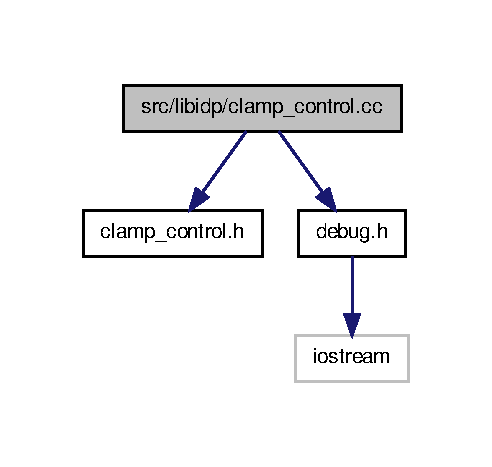
\includegraphics[width=236pt]{clamp__control_8cc__incl}
\end{center}
\end{figure}
\subsection*{Namespaces}
\begin{DoxyCompactItemize}
\item 
namespace \hyperlink{namespaceIDP}{IDP}
\end{DoxyCompactItemize}
\subsection*{Defines}
\begin{DoxyCompactItemize}
\item 
\#define \hyperlink{clamp__control_8cc_a14ded244c47bbba850a8a4be6d16c7e3}{MODULE\_\-NAME}~\char`\"{}Clamp\char`\"{}
\item 
\#define \hyperlink{clamp__control_8cc_ae04c5e41f64b51d21bc71565938a59d6}{TRACE\_\-ENABLED}~false
\item 
\#define \hyperlink{clamp__control_8cc_a7d2ae674cad5299a52b0e7dceac10087}{DEBUG\_\-ENABLED}~true
\item 
\#define \hyperlink{clamp__control_8cc_a580f977f97ee7f7ceb91b1c42306f537}{INFO\_\-ENABLED}~true
\item 
\#define \hyperlink{clamp__control_8cc_a292d4ca4e07d63502916a17a853ab606}{ERROR\_\-ENABLED}~true
\end{DoxyCompactItemize}


\subsection{Define Documentation}
\hypertarget{clamp__control_8cc_a7d2ae674cad5299a52b0e7dceac10087}{
\index{clamp\_\-control.cc@{clamp\_\-control.cc}!DEBUG\_\-ENABLED@{DEBUG\_\-ENABLED}}
\index{DEBUG\_\-ENABLED@{DEBUG\_\-ENABLED}!clamp_control.cc@{clamp\_\-control.cc}}
\subsubsection[{DEBUG\_\-ENABLED}]{\setlength{\rightskip}{0pt plus 5cm}\#define DEBUG\_\-ENABLED~true}}
\label{clamp__control_8cc_a7d2ae674cad5299a52b0e7dceac10087}


Definition at line 12 of file clamp\_\-control.cc.

\hypertarget{clamp__control_8cc_a292d4ca4e07d63502916a17a853ab606}{
\index{clamp\_\-control.cc@{clamp\_\-control.cc}!ERROR\_\-ENABLED@{ERROR\_\-ENABLED}}
\index{ERROR\_\-ENABLED@{ERROR\_\-ENABLED}!clamp_control.cc@{clamp\_\-control.cc}}
\subsubsection[{ERROR\_\-ENABLED}]{\setlength{\rightskip}{0pt plus 5cm}\#define ERROR\_\-ENABLED~true}}
\label{clamp__control_8cc_a292d4ca4e07d63502916a17a853ab606}


Definition at line 14 of file clamp\_\-control.cc.

\hypertarget{clamp__control_8cc_a580f977f97ee7f7ceb91b1c42306f537}{
\index{clamp\_\-control.cc@{clamp\_\-control.cc}!INFO\_\-ENABLED@{INFO\_\-ENABLED}}
\index{INFO\_\-ENABLED@{INFO\_\-ENABLED}!clamp_control.cc@{clamp\_\-control.cc}}
\subsubsection[{INFO\_\-ENABLED}]{\setlength{\rightskip}{0pt plus 5cm}\#define INFO\_\-ENABLED~true}}
\label{clamp__control_8cc_a580f977f97ee7f7ceb91b1c42306f537}


Definition at line 13 of file clamp\_\-control.cc.

\hypertarget{clamp__control_8cc_a14ded244c47bbba850a8a4be6d16c7e3}{
\index{clamp\_\-control.cc@{clamp\_\-control.cc}!MODULE\_\-NAME@{MODULE\_\-NAME}}
\index{MODULE\_\-NAME@{MODULE\_\-NAME}!clamp_control.cc@{clamp\_\-control.cc}}
\subsubsection[{MODULE\_\-NAME}]{\setlength{\rightskip}{0pt plus 5cm}\#define MODULE\_\-NAME~\char`\"{}Clamp\char`\"{}}}
\label{clamp__control_8cc_a14ded244c47bbba850a8a4be6d16c7e3}


Definition at line 10 of file clamp\_\-control.cc.

\hypertarget{clamp__control_8cc_ae04c5e41f64b51d21bc71565938a59d6}{
\index{clamp\_\-control.cc@{clamp\_\-control.cc}!TRACE\_\-ENABLED@{TRACE\_\-ENABLED}}
\index{TRACE\_\-ENABLED@{TRACE\_\-ENABLED}!clamp_control.cc@{clamp\_\-control.cc}}
\subsubsection[{TRACE\_\-ENABLED}]{\setlength{\rightskip}{0pt plus 5cm}\#define TRACE\_\-ENABLED~false}}
\label{clamp__control_8cc_ae04c5e41f64b51d21bc71565938a59d6}


Definition at line 11 of file clamp\_\-control.cc.


\hypertarget{clamp__control_8h}{
\section{libidp/clamp\_\-control.h File Reference}
\label{clamp__control_8h}\index{libidp/clamp\_\-control.h@{libidp/clamp\_\-control.h}}
}
This graph shows which files directly or indirectly include this file:\nopagebreak
\begin{figure}[H]
\begin{center}
\leavevmode
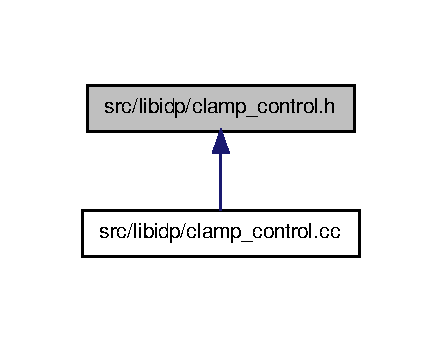
\includegraphics[width=196pt]{clamp__control_8h__dep__incl}
\end{center}
\end{figure}
\subsection*{Classes}
\begin{DoxyCompactItemize}
\item 
class \hyperlink{classIDP_1_1ClampControl}{IDP::ClampControl}
\begin{DoxyCompactList}\small\item\em Manage the actuation of the clamp, as well as the detection and analysis of bobbins for their colour and badness. \item\end{DoxyCompactList}\end{DoxyCompactItemize}
\subsection*{Namespaces}
\begin{DoxyCompactItemize}
\item 
namespace \hyperlink{namespaceIDP}{IDP}
\end{DoxyCompactItemize}
\subsection*{Enumerations}
\begin{DoxyCompactItemize}
\item 
enum \hyperlink{namespaceIDP_a6efd2cca14c0dae1c6458714ce0218df}{IDP::BobbinColour} \{ \hyperlink{namespaceIDP_a6efd2cca14c0dae1c6458714ce0218dfa1bbb59488c1d089eefb9b54146bcdb26}{IDP::BOBBIN\_\-RED}, 
\hyperlink{namespaceIDP_a6efd2cca14c0dae1c6458714ce0218dfa047d7c5fcd5669f1a819d05fb5319f0b}{IDP::BOBBIN\_\-GREEN}, 
\hyperlink{namespaceIDP_a6efd2cca14c0dae1c6458714ce0218dfa8f427bfb1c335650a7ada595e1607d00}{IDP::BOBBIN\_\-WHITE}
 \}
\item 
enum \hyperlink{namespaceIDP_adf12b2c1e1c228810b18c34a3c88c32d}{IDP::BobbinBadness} \{ \hyperlink{namespaceIDP_adf12b2c1e1c228810b18c34a3c88c32dafdc1b8b5a9d849fd99ac2ae438b632dd}{IDP::BOBBIN\_\-GOOD}, 
\hyperlink{namespaceIDP_adf12b2c1e1c228810b18c34a3c88c32da6cb4993a316e9d4dc9836d3d990fd0f6}{IDP::BOBBIN\_\-BAD}
 \}
\end{DoxyCompactItemize}

\hypertarget{debug_8h}{
\section{src/libidp/debug.h File Reference}
\label{debug_8h}\index{src/libidp/debug.h@{src/libidp/debug.h}}
}
{\ttfamily \#include $<$iostream$>$}\par
Include dependency graph for debug.h:\nopagebreak
\begin{figure}[H]
\begin{center}
\leavevmode
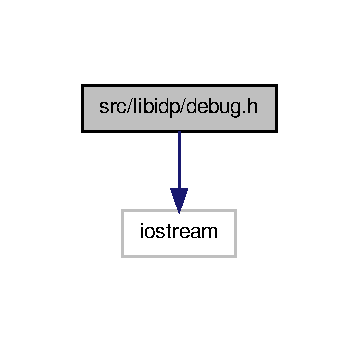
\includegraphics[width=172pt]{debug_8h__incl}
\end{center}
\end{figure}
This graph shows which files directly or indirectly include this file:
\nopagebreak
\begin{figure}[H]
\begin{center}
\leavevmode
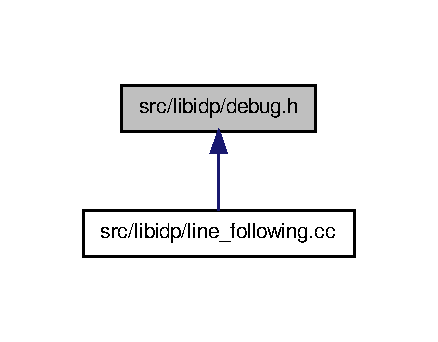
\includegraphics[width=400pt]{debug_8h__dep__incl}
\end{center}
\end{figure}

\hypertarget{hal_8cc}{
\section{src/libidp/hal.cc File Reference}
\label{hal_8cc}\index{src/libidp/hal.cc@{src/libidp/hal.cc}}
}
{\ttfamily \#include \char`\"{}hal.h\char`\"{}}\par
{\ttfamily \#include $<$iostream$>$}\par
{\ttfamily \#include $<$cstdlib$>$}\par
{\ttfamily \#include $<$robot\_\-instr.h$>$}\par
{\ttfamily \#include \char`\"{}debug.h\char`\"{}}\par
Include dependency graph for hal.cc:
\nopagebreak
\begin{figure}[H]
\begin{center}
\leavevmode
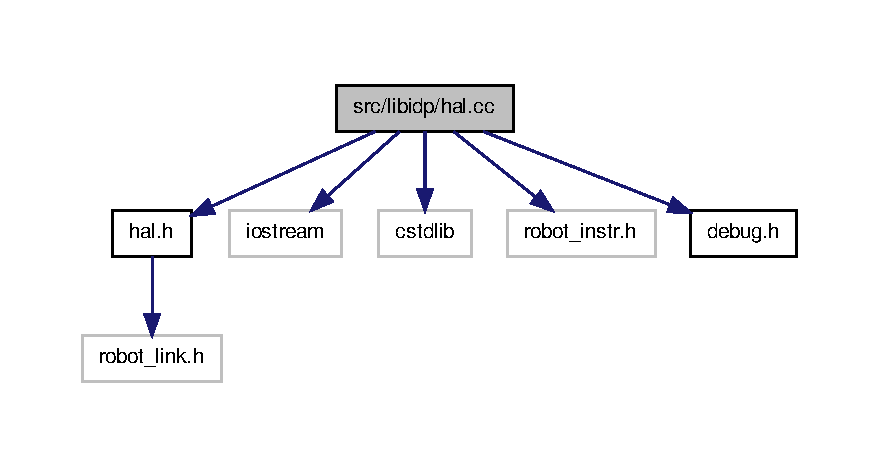
\includegraphics[width=388pt]{hal_8cc__incl}
\end{center}
\end{figure}
\subsection*{Namespaces}
\begin{DoxyCompactItemize}
\item 
namespace \hyperlink{namespaceIDP}{IDP}
\end{DoxyCompactItemize}
\subsection*{Defines}
\begin{DoxyCompactItemize}
\item 
\#define \hyperlink{hal_8cc_a14ded244c47bbba850a8a4be6d16c7e3}{MODULE\_\-NAME}~\char`\"{}HAL\char`\"{}
\item 
\#define \hyperlink{hal_8cc_ae04c5e41f64b51d21bc71565938a59d6}{TRACE\_\-ENABLED}~false
\item 
\#define \hyperlink{hal_8cc_a7d2ae674cad5299a52b0e7dceac10087}{DEBUG\_\-ENABLED}~false
\item 
\#define \hyperlink{hal_8cc_a580f977f97ee7f7ceb91b1c42306f537}{INFO\_\-ENABLED}~true
\item 
\#define \hyperlink{hal_8cc_a292d4ca4e07d63502916a17a853ab606}{ERROR\_\-ENABLED}~true
\item 
\#define \hyperlink{hal_8cc_a86d500a34c624c2cae56bc25a31b12f3}{UNUSED}(x)~(void)(x)
\end{DoxyCompactItemize}


\subsection{Define Documentation}
\hypertarget{hal_8cc_a7d2ae674cad5299a52b0e7dceac10087}{
\index{hal.cc@{hal.cc}!DEBUG\_\-ENABLED@{DEBUG\_\-ENABLED}}
\index{DEBUG\_\-ENABLED@{DEBUG\_\-ENABLED}!hal.cc@{hal.cc}}
\subsubsection[{DEBUG\_\-ENABLED}]{\setlength{\rightskip}{0pt plus 5cm}\#define DEBUG\_\-ENABLED~false}}
\label{hal_8cc_a7d2ae674cad5299a52b0e7dceac10087}


Definition at line 17 of file hal.cc.

\hypertarget{hal_8cc_a292d4ca4e07d63502916a17a853ab606}{
\index{hal.cc@{hal.cc}!ERROR\_\-ENABLED@{ERROR\_\-ENABLED}}
\index{ERROR\_\-ENABLED@{ERROR\_\-ENABLED}!hal.cc@{hal.cc}}
\subsubsection[{ERROR\_\-ENABLED}]{\setlength{\rightskip}{0pt plus 5cm}\#define ERROR\_\-ENABLED~true}}
\label{hal_8cc_a292d4ca4e07d63502916a17a853ab606}


Definition at line 19 of file hal.cc.

\hypertarget{hal_8cc_a580f977f97ee7f7ceb91b1c42306f537}{
\index{hal.cc@{hal.cc}!INFO\_\-ENABLED@{INFO\_\-ENABLED}}
\index{INFO\_\-ENABLED@{INFO\_\-ENABLED}!hal.cc@{hal.cc}}
\subsubsection[{INFO\_\-ENABLED}]{\setlength{\rightskip}{0pt plus 5cm}\#define INFO\_\-ENABLED~true}}
\label{hal_8cc_a580f977f97ee7f7ceb91b1c42306f537}


Definition at line 18 of file hal.cc.

\hypertarget{hal_8cc_a14ded244c47bbba850a8a4be6d16c7e3}{
\index{hal.cc@{hal.cc}!MODULE\_\-NAME@{MODULE\_\-NAME}}
\index{MODULE\_\-NAME@{MODULE\_\-NAME}!hal.cc@{hal.cc}}
\subsubsection[{MODULE\_\-NAME}]{\setlength{\rightskip}{0pt plus 5cm}\#define MODULE\_\-NAME~\char`\"{}HAL\char`\"{}}}
\label{hal_8cc_a14ded244c47bbba850a8a4be6d16c7e3}


Definition at line 15 of file hal.cc.

\hypertarget{hal_8cc_ae04c5e41f64b51d21bc71565938a59d6}{
\index{hal.cc@{hal.cc}!TRACE\_\-ENABLED@{TRACE\_\-ENABLED}}
\index{TRACE\_\-ENABLED@{TRACE\_\-ENABLED}!hal.cc@{hal.cc}}
\subsubsection[{TRACE\_\-ENABLED}]{\setlength{\rightskip}{0pt plus 5cm}\#define TRACE\_\-ENABLED~false}}
\label{hal_8cc_ae04c5e41f64b51d21bc71565938a59d6}


Definition at line 16 of file hal.cc.

\hypertarget{hal_8cc_a86d500a34c624c2cae56bc25a31b12f3}{
\index{hal.cc@{hal.cc}!UNUSED@{UNUSED}}
\index{UNUSED@{UNUSED}!hal.cc@{hal.cc}}
\subsubsection[{UNUSED}]{\setlength{\rightskip}{0pt plus 5cm}\#define UNUSED(
\begin{DoxyParamCaption}
\item[{}]{x}
\end{DoxyParamCaption}
)~(void)(x)}}
\label{hal_8cc_a86d500a34c624c2cae56bc25a31b12f3}


Definition at line 23 of file hal.cc.


\hypertarget{hal_8h}{
\section{src/libidp/hal.h File Reference}
\label{hal_8h}\index{src/libidp/hal.h@{src/libidp/hal.h}}
}
{\ttfamily \#include $<$robot\_\-link.h$>$}\par
Include dependency graph for hal.h:\nopagebreak
\begin{figure}[H]
\begin{center}
\leavevmode
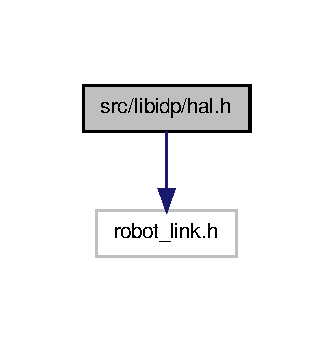
\includegraphics[width=160pt]{hal_8h__incl}
\end{center}
\end{figure}
This graph shows which files directly or indirectly include this file:\nopagebreak
\begin{figure}[H]
\begin{center}
\leavevmode
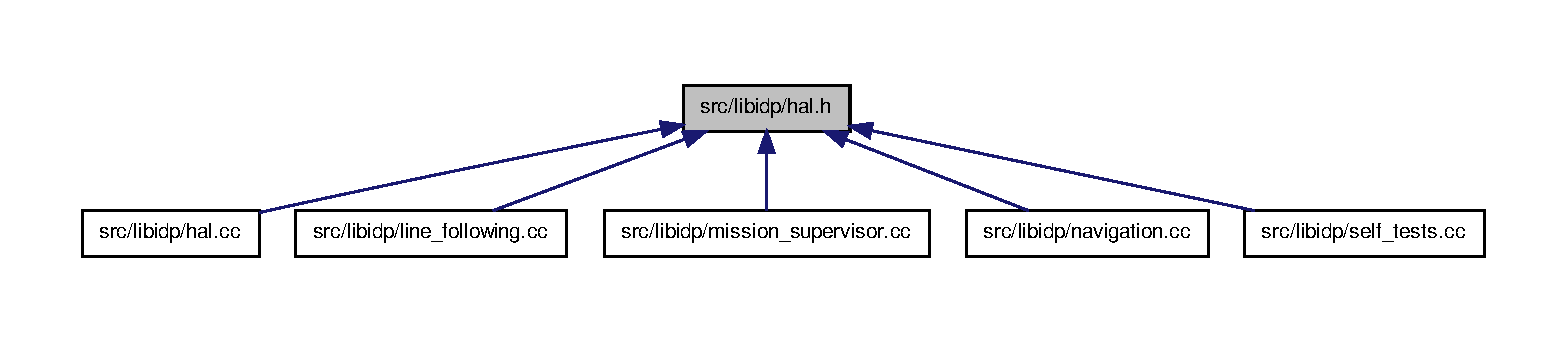
\includegraphics[width=400pt]{hal_8h__dep__incl}
\end{center}
\end{figure}
\subsection*{Classes}
\begin{DoxyCompactItemize}
\item 
struct \hyperlink{structIDP_1_1LineSensors}{IDP::LineSensors}
\begin{DoxyCompactList}\small\item\em Contains the LINE or NO\_\-LINE status of each of the four IR sensors used for line following. \item\end{DoxyCompactList}\item 
class \hyperlink{classIDP_1_1HardwareAbstractionLayer}{IDP::HardwareAbstractionLayer}
\begin{DoxyCompactList}\small\item\em Provide a hardware agnostic interface to the required hardware functionality. \item\end{DoxyCompactList}\end{DoxyCompactItemize}
\subsection*{Namespaces}
\begin{DoxyCompactItemize}
\item 
namespace \hyperlink{namespaceIDP}{IDP}


\begin{DoxyCompactList}\small\item\em Contains all the \hyperlink{namespaceIDP}{IDP} related functionality including libidp and some idpbin classes. \item\end{DoxyCompactList}

\end{DoxyCompactItemize}
\subsection*{Enumerations}
\begin{DoxyCompactItemize}
\item 
enum \hyperlink{namespaceIDP_afc3b1d4cbb313bfc854f49d6f23b25f7}{IDP::LineSensorStatus} \{ \hyperlink{namespaceIDP_afc3b1d4cbb313bfc854f49d6f23b25f7ab8f6b528c0b2fd3edfdd6463cc6a2fd2}{IDP::LINE}, 
\hyperlink{namespaceIDP_afc3b1d4cbb313bfc854f49d6f23b25f7a8f85d4834fc4519df3f2053201d497d1}{IDP::NO\_\-LINE}
 \}
\begin{DoxyCompactList}\small\item\em Line sensor status, LINE or NO\_\-LINE. \item\end{DoxyCompactList}\end{DoxyCompactItemize}
\subsection*{Variables}
\begin{DoxyCompactItemize}
\item 
const int \hyperlink{namespaceIDP_a4ead0b21ad2c507b542445695182d4cd}{IDP::MOTOR\_\-MAX\_\-SPEED} = 127
\begin{DoxyCompactList}\small\item\em Highest allowable motor speed in either direction. \item\end{DoxyCompactList}\item 
const int \hyperlink{namespaceIDP_ab3a00a6cc8a6dba271e38d337daf4703}{IDP::MOTOR\_\-RAMP\_\-TIME} = 16
\begin{DoxyCompactList}\small\item\em How fast to ramp the motors towards the desired speed. \item\end{DoxyCompactList}\end{DoxyCompactItemize}

\hypertarget{libidp_8h}{
\section{libidp/libidp.h File Reference}
\label{libidp_8h}\index{libidp/libidp.h@{libidp/libidp.h}}
}
{\ttfamily \#include \char`\"{}mission\_\-supervisor.h\char`\"{}}\par
Include dependency graph for libidp.h:

\hypertarget{line__following_8cc}{
\section{libidp/line\_\-following.cc File Reference}
\label{line__following_8cc}\index{libidp/line\_\-following.cc@{libidp/line\_\-following.cc}}
}
{\ttfamily \#include $<$iostream$>$}\par
{\ttfamily \#include $<$robot\_\-instr.h$>$}\par
{\ttfamily \#include \char`\"{}hal.h\char`\"{}}\par
{\ttfamily \#include \char`\"{}line\_\-following.h\char`\"{}}\par
Include dependency graph for line\_\-following.cc:
\nopagebreak
\begin{figure}[H]
\begin{center}
\leavevmode
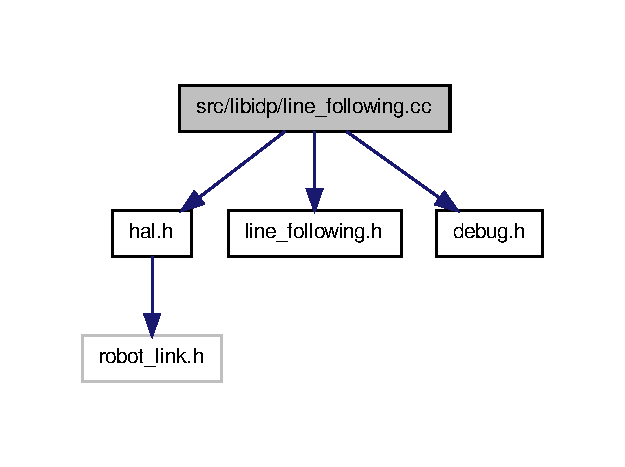
\includegraphics[width=378pt]{line__following_8cc__incl}
\end{center}
\end{figure}
\subsection*{Namespaces}
\begin{DoxyCompactItemize}
\item 
namespace \hyperlink{namespaceIDP}{IDP}
\end{DoxyCompactItemize}

\hypertarget{line__following_8h}{
\section{libidp/line\_\-following.h File Reference}
\label{line__following_8h}\index{libidp/line\_\-following.h@{libidp/line\_\-following.h}}
}
{\ttfamily \#include $<$robot\_\-link.h$>$}\par
Include dependency graph for line\_\-following.h:\nopagebreak
\begin{figure}[H]
\begin{center}
\leavevmode
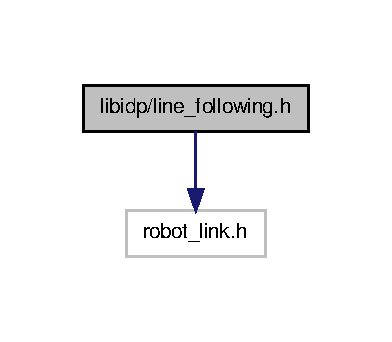
\includegraphics[width=188pt]{line__following_8h__incl}
\end{center}
\end{figure}
This graph shows which files directly or indirectly include this file:\nopagebreak
\begin{figure}[H]
\begin{center}
\leavevmode
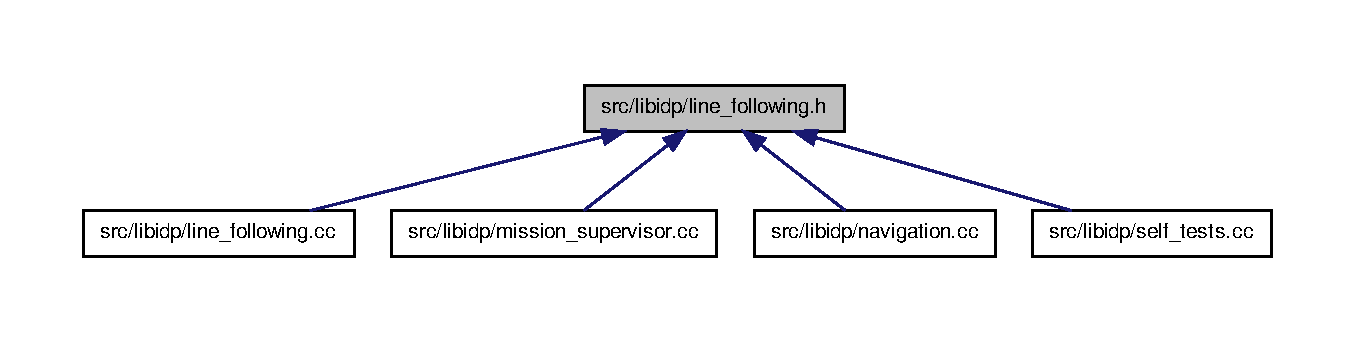
\includegraphics[width=400pt]{line__following_8h__dep__incl}
\end{center}
\end{figure}
\subsection*{Classes}
\begin{DoxyCompactItemize}
\item 
class \hyperlink{classIDP_1_1LineFollowing}{IDP::LineFollowing}
\begin{DoxyCompactList}\small\item\em Maintain the robot position correctly with respect to the white line markers, during driving and manouvering. \item\end{DoxyCompactList}\end{DoxyCompactItemize}
\subsection*{Namespaces}
\begin{DoxyCompactItemize}
\item 
namespace \hyperlink{namespaceIDP}{IDP}
\end{DoxyCompactItemize}
\subsection*{Variables}
\begin{DoxyCompactItemize}
\item 
const double \hyperlink{namespaceIDP_aa2b933f600179026dbca5d8bc63c3baf}{IDP::ki} = 4.0
\end{DoxyCompactItemize}

\hypertarget{mission__supervisor_8cc}{
\section{libidp/mission\_\-supervisor.cc File Reference}
\label{mission__supervisor_8cc}\index{libidp/mission\_\-supervisor.cc@{libidp/mission\_\-supervisor.cc}}
}
{\ttfamily \#include \char`\"{}mission\_\-supervisor.h\char`\"{}}\par
{\ttfamily \#include $<$iostream$>$}\par
{\ttfamily \#include $<$robot\_\-instr.h$>$}\par
{\ttfamily \#include \char`\"{}hal.h\char`\"{}}\par
{\ttfamily \#include \char`\"{}line\_\-following.h\char`\"{}}\par
Include dependency graph for mission\_\-supervisor.cc:
\subsection*{Namespaces}
\begin{DoxyCompactItemize}
\item 
namespace \hyperlink{namespaceIDP}{IDP}
\end{DoxyCompactItemize}

\hypertarget{mission__supervisor_8h}{
\section{libidp/mission\_\-supervisor.h File Reference}
\label{mission__supervisor_8h}\index{libidp/mission\_\-supervisor.h@{libidp/mission\_\-supervisor.h}}
}
{\ttfamily \#include $<$robot\_\-link.h$>$}\par
Include dependency graph for mission\_\-supervisor.h:
This graph shows which files directly or indirectly include this file:
\subsection*{Classes}
\begin{DoxyCompactItemize}
\item 
class \hyperlink{classIDP_1_1MissionSupervisor}{IDP::MissionSupervisor}
\end{DoxyCompactItemize}
\subsection*{Namespaces}
\begin{DoxyCompactItemize}
\item 
namespace \hyperlink{namespaceIDP}{IDP}
\end{DoxyCompactItemize}

\hypertarget{navigation_8cc}{
\section{src/libidp/navigation.cc File Reference}
\label{navigation_8cc}\index{src/libidp/navigation.cc@{src/libidp/navigation.cc}}
}
{\ttfamily \#include \char`\"{}navigation.h\char`\"{}}\par
{\ttfamily \#include \char`\"{}line\_\-following.h\char`\"{}}\par
{\ttfamily \#include \char`\"{}hal.h\char`\"{}}\par
{\ttfamily \#include \char`\"{}debug.h\char`\"{}}\par
Include dependency graph for navigation.cc:\nopagebreak
\begin{figure}[H]
\begin{center}
\leavevmode
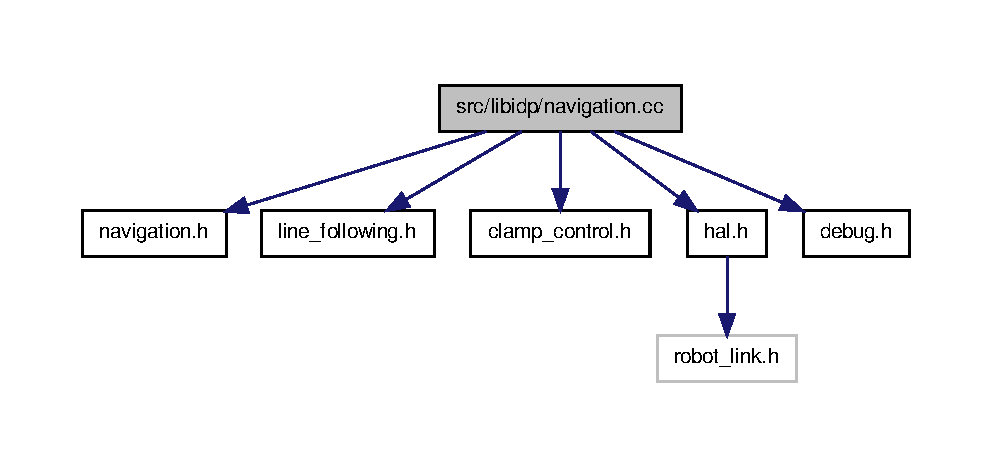
\includegraphics[width=386pt]{navigation_8cc__incl}
\end{center}
\end{figure}
\subsection*{Namespaces}
\begin{DoxyCompactItemize}
\item 
namespace \hyperlink{namespaceIDP}{IDP}


\begin{DoxyCompactList}\small\item\em Contains all the \hyperlink{namespaceIDP}{IDP} related functionality including libidp and some idpbin classes. \item\end{DoxyCompactList}

\end{DoxyCompactItemize}
\subsection*{Defines}
\begin{DoxyCompactItemize}
\item 
\#define \hyperlink{navigation_8cc_a14ded244c47bbba850a8a4be6d16c7e3}{MODULE\_\-NAME}~\char`\"{}Navigation\char`\"{}
\item 
\#define \hyperlink{navigation_8cc_ae04c5e41f64b51d21bc71565938a59d6}{TRACE\_\-ENABLED}~true
\item 
\#define \hyperlink{navigation_8cc_a7d2ae674cad5299a52b0e7dceac10087}{DEBUG\_\-ENABLED}~true
\item 
\#define \hyperlink{navigation_8cc_a580f977f97ee7f7ceb91b1c42306f537}{INFO\_\-ENABLED}~true
\item 
\#define \hyperlink{navigation_8cc_a292d4ca4e07d63502916a17a853ab606}{ERROR\_\-ENABLED}~true
\item 
\#define \hyperlink{navigation_8cc_a86d500a34c624c2cae56bc25a31b12f3}{UNUSED}(x)~(void)(x)
\end{DoxyCompactItemize}
\subsection*{Variables}
\begin{DoxyCompactItemize}
\item 
const NavigationTurn \hyperlink{namespaceIDP_aa117cb76acf18e6af22830d5f2468ff4}{IDP::NAVIGATION\_\-NODE\_\-TURNS} \mbox{[}MAX\_\-DIRECTION\mbox{]}\mbox{[}MAX\_\-NODE\mbox{]}
\begin{DoxyCompactList}\small\item\em The turns at each node. \item\end{DoxyCompactList}\item 
const NavigationTurn \hyperlink{namespaceIDP_a0bada0608b684564e235786b3b38c10a}{IDP::NAVIGATION\_\-TURN\_\-MAP} \mbox{[}MAX\_\-DIRECTION\mbox{]}\mbox{[}MAX\_\-NODE\mbox{]}
\begin{DoxyCompactList}\small\item\em Turns that should be taken at each node in each direction. \item\end{DoxyCompactList}\item 
const NavigationNode \hyperlink{namespaceIDP_a33e1b72d66088b211bfeb61b18d7b63b}{IDP::NAVIGATION\_\-LOCATION\_\-LOOKUP} \mbox{[}MAX\_\-LOCATION\mbox{]}\mbox{[}2\mbox{]}
\begin{DoxyCompactList}\small\item\em The lookup table of NavigationLocations to a pair of NavigationNodes indicating the start and end node (with implied direction). \item\end{DoxyCompactList}\item 
const NavigationNode \hyperlink{namespaceIDP_a33ba7fcc78e0c8e5477d2ed6ac18e48f}{IDP::NAVIGATION\_\-ROUTE\_\-MAP} \mbox{[}MAX\_\-DIRECTION\mbox{]}\mbox{[}MAX\_\-NODE\mbox{]}
\begin{DoxyCompactList}\small\item\em The route to take, node by node. \item\end{DoxyCompactList}\end{DoxyCompactItemize}


\subsection{Define Documentation}
\hypertarget{navigation_8cc_a7d2ae674cad5299a52b0e7dceac10087}{
\index{navigation.cc@{navigation.cc}!DEBUG\_\-ENABLED@{DEBUG\_\-ENABLED}}
\index{DEBUG\_\-ENABLED@{DEBUG\_\-ENABLED}!navigation.cc@{navigation.cc}}
\subsubsection[{DEBUG\_\-ENABLED}]{\setlength{\rightskip}{0pt plus 5cm}\#define DEBUG\_\-ENABLED~true}}
\label{navigation_8cc_a7d2ae674cad5299a52b0e7dceac10087}


Definition at line 14 of file navigation.cc.

\hypertarget{navigation_8cc_a292d4ca4e07d63502916a17a853ab606}{
\index{navigation.cc@{navigation.cc}!ERROR\_\-ENABLED@{ERROR\_\-ENABLED}}
\index{ERROR\_\-ENABLED@{ERROR\_\-ENABLED}!navigation.cc@{navigation.cc}}
\subsubsection[{ERROR\_\-ENABLED}]{\setlength{\rightskip}{0pt plus 5cm}\#define ERROR\_\-ENABLED~true}}
\label{navigation_8cc_a292d4ca4e07d63502916a17a853ab606}


Definition at line 16 of file navigation.cc.

\hypertarget{navigation_8cc_a580f977f97ee7f7ceb91b1c42306f537}{
\index{navigation.cc@{navigation.cc}!INFO\_\-ENABLED@{INFO\_\-ENABLED}}
\index{INFO\_\-ENABLED@{INFO\_\-ENABLED}!navigation.cc@{navigation.cc}}
\subsubsection[{INFO\_\-ENABLED}]{\setlength{\rightskip}{0pt plus 5cm}\#define INFO\_\-ENABLED~true}}
\label{navigation_8cc_a580f977f97ee7f7ceb91b1c42306f537}


Definition at line 15 of file navigation.cc.

\hypertarget{navigation_8cc_a14ded244c47bbba850a8a4be6d16c7e3}{
\index{navigation.cc@{navigation.cc}!MODULE\_\-NAME@{MODULE\_\-NAME}}
\index{MODULE\_\-NAME@{MODULE\_\-NAME}!navigation.cc@{navigation.cc}}
\subsubsection[{MODULE\_\-NAME}]{\setlength{\rightskip}{0pt plus 5cm}\#define MODULE\_\-NAME~\char`\"{}Navigation\char`\"{}}}
\label{navigation_8cc_a14ded244c47bbba850a8a4be6d16c7e3}


Definition at line 12 of file navigation.cc.

\hypertarget{navigation_8cc_ae04c5e41f64b51d21bc71565938a59d6}{
\index{navigation.cc@{navigation.cc}!TRACE\_\-ENABLED@{TRACE\_\-ENABLED}}
\index{TRACE\_\-ENABLED@{TRACE\_\-ENABLED}!navigation.cc@{navigation.cc}}
\subsubsection[{TRACE\_\-ENABLED}]{\setlength{\rightskip}{0pt plus 5cm}\#define TRACE\_\-ENABLED~true}}
\label{navigation_8cc_ae04c5e41f64b51d21bc71565938a59d6}


Definition at line 13 of file navigation.cc.

\hypertarget{navigation_8cc_a86d500a34c624c2cae56bc25a31b12f3}{
\index{navigation.cc@{navigation.cc}!UNUSED@{UNUSED}}
\index{UNUSED@{UNUSED}!navigation.cc@{navigation.cc}}
\subsubsection[{UNUSED}]{\setlength{\rightskip}{0pt plus 5cm}\#define UNUSED(
\begin{DoxyParamCaption}
\item[{}]{x}
\end{DoxyParamCaption}
)~(void)(x)}}
\label{navigation_8cc_a86d500a34c624c2cae56bc25a31b12f3}


Definition at line 20 of file navigation.cc.


\hypertarget{navigation_8h}{
\section{src/libidp/navigation.h File Reference}
\label{navigation_8h}\index{src/libidp/navigation.h@{src/libidp/navigation.h}}
}
This graph shows which files directly or indirectly include this file:\nopagebreak
\begin{figure}[H]
\begin{center}
\leavevmode
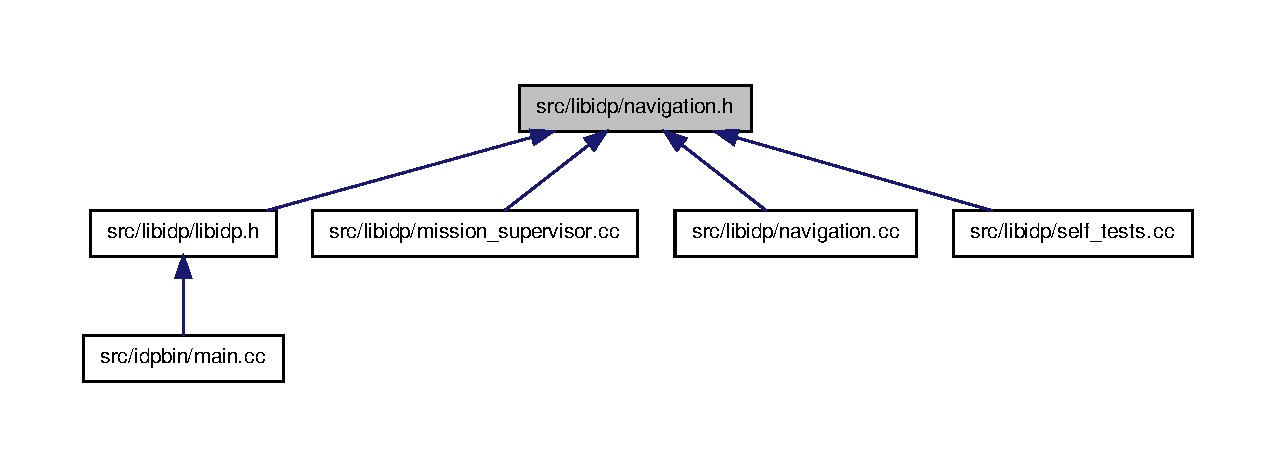
\includegraphics[width=400pt]{navigation_8h__dep__incl}
\end{center}
\end{figure}
\subsection*{Classes}
\begin{DoxyCompactItemize}
\item 
class \hyperlink{classIDP_1_1Navigation}{IDP::Navigation}
\begin{DoxyCompactList}\small\item\em Find a route from one place to another on the board, and maintain an estimate of the current position. \item\end{DoxyCompactList}\end{DoxyCompactItemize}
\subsection*{Namespaces}
\begin{DoxyCompactItemize}
\item 
namespace \hyperlink{namespaceIDP}{IDP}


\begin{DoxyCompactList}\small\item\em Contains all the \hyperlink{namespaceIDP}{IDP} related functionality including libidp and some idpbin classes. \item\end{DoxyCompactList}

\end{DoxyCompactItemize}
\subsection*{Enumerations}
\begin{DoxyCompactItemize}
\item 
enum \hyperlink{namespaceIDP_a1a96e566e4d675fdf20780cc96d92283}{IDP::NavigationStatus} \{ \hyperlink{namespaceIDP_a1a96e566e4d675fdf20780cc96d92283a9f52fe7970aefcb1b74e9aea3798f39d}{IDP::NAVIGATION\_\-ENROUTE}, 
\hyperlink{namespaceIDP_a1a96e566e4d675fdf20780cc96d92283ab9e83c995cb23a5782b23b198dcbabcb}{IDP::NAVIGATION\_\-ARRIVED}, 
\hyperlink{namespaceIDP_a1a96e566e4d675fdf20780cc96d92283ad75d1c5522e0a38dbe62266912d411ba}{IDP::NAVIGATION\_\-LOST}, 
\hyperlink{namespaceIDP_a1a96e566e4d675fdf20780cc96d92283a6911d3c0411bacf5135884884fb86093}{IDP::MAX\_\-STATUS}
 \}
\begin{DoxyCompactList}\small\item\em Current navigation status. \item\end{DoxyCompactList}\item 
enum \hyperlink{namespaceIDP_ab9c412f0fd539b5d70385066c30465a0}{IDP::NavigationLocation} \{ \hyperlink{namespaceIDP_ab9c412f0fd539b5d70385066c30465a0a0cfb642ce5e4133706998843eb3c8da1}{IDP::NAVIGATION\_\-BOXES}, 
\hyperlink{namespaceIDP_ab9c412f0fd539b5d70385066c30465a0af1bde0912725a75705d0fb74637f20c1}{IDP::NAVIGATION\_\-RACK}, 
\hyperlink{namespaceIDP_ab9c412f0fd539b5d70385066c30465a0a10e09a3f2969d951f0dc233cb76eb4bf}{IDP::NAVIGATION\_\-DELIVERY}, 
\hyperlink{namespaceIDP_ab9c412f0fd539b5d70385066c30465a0a4db81c4e7223eb8250c3575d1962241d}{IDP::MAX\_\-LOCATION}
 \}
\begin{DoxyCompactList}\small\item\em Possible locations for navigation to be asked to go to. \item\end{DoxyCompactList}\item 
enum \hyperlink{namespaceIDP_a899dbbc9d55dd4919ded1859281f503d}{IDP::NavigationDirection} \{ \hyperlink{namespaceIDP_a899dbbc9d55dd4919ded1859281f503daf54b8983cf0d707430d34ada92ded9f6}{IDP::NAVIGATION\_\-CLOCKWISE}, 
\hyperlink{namespaceIDP_a899dbbc9d55dd4919ded1859281f503da63c9c55ca2ca92e66c0959dc14c19d4e}{IDP::NAVIGATION\_\-ANTICLOCKWISE}, 
\hyperlink{namespaceIDP_a899dbbc9d55dd4919ded1859281f503da71609a18cba61e0b52f3f5de70e307d8}{IDP::MAX\_\-DIRECTION}
 \}
\begin{DoxyCompactList}\small\item\em Directions around the circuit. \item\end{DoxyCompactList}\item 
enum \hyperlink{namespaceIDP_a286f26dda01010063dff761803b4cd16}{IDP::NavigationNode} \{ \par
\hyperlink{namespaceIDP_a286f26dda01010063dff761803b4cd16a01e42e06cc228327ff3d4288b7c416a7}{IDP::NODE1}, 
\hyperlink{namespaceIDP_a286f26dda01010063dff761803b4cd16a643f7b9d84010cdf26d3245b52e95d61}{IDP::NODE2}, 
\hyperlink{namespaceIDP_a286f26dda01010063dff761803b4cd16ad8c020bde6a1a7b8ec426cea377c3220}{IDP::NODE3}, 
\hyperlink{namespaceIDP_a286f26dda01010063dff761803b4cd16a52a02df944cc115f43d73ce2a3fb206a}{IDP::NODE4}, 
\par
\hyperlink{namespaceIDP_a286f26dda01010063dff761803b4cd16a25b67ea21e28e6928e61191d8d85aee9}{IDP::NODE5}, 
\hyperlink{namespaceIDP_a286f26dda01010063dff761803b4cd16a82c1907a7289c9ae600c7597640c7999}{IDP::NODE6}, 
\hyperlink{namespaceIDP_a286f26dda01010063dff761803b4cd16a64ef68f9f4ffd2a6b200d9667ae5ff69}{IDP::NODE7}, 
\hyperlink{namespaceIDP_a286f26dda01010063dff761803b4cd16af0865100370f00bba081b38a771aac19}{IDP::NODE8}, 
\par
\hyperlink{namespaceIDP_a286f26dda01010063dff761803b4cd16ae3e2ad58c131978b30cb565da7a28cce}{IDP::NODE9}, 
\hyperlink{namespaceIDP_a286f26dda01010063dff761803b4cd16ac1ad66fa991f24bbd3b7d38935ffefc3}{IDP::NODE10}, 
\hyperlink{namespaceIDP_a286f26dda01010063dff761803b4cd16affbfbc02ea10aa15e24d64ed5cb70ea0}{IDP::NODE11}, 
\hyperlink{namespaceIDP_a286f26dda01010063dff761803b4cd16a9d305178c7e7907ce612388ff08063c4}{IDP::MAX\_\-NODE}
 \}
\begin{DoxyCompactList}\small\item\em Navigation nodes, numbered clockwise from the bottom right corner of the table. \item\end{DoxyCompactList}\item 
enum \hyperlink{namespaceIDP_ab8b8e9ff9f7de27da30c1fffaeef4b72}{IDP::NavigationTurn} \{ \par
\hyperlink{namespaceIDP_ab8b8e9ff9f7de27da30c1fffaeef4b72a89e423fa73cc15b78c7a12d75358bc5d}{IDP::STRAIGHT}, 
\hyperlink{namespaceIDP_ab8b8e9ff9f7de27da30c1fffaeef4b72a06987c9e055bf2a24b28c83d93462f75}{IDP::LEFT}, 
\hyperlink{namespaceIDP_ab8b8e9ff9f7de27da30c1fffaeef4b72accfe3edbad6f4b3795cee55d550c77da}{IDP::RIGHT}, 
\hyperlink{namespaceIDP_ab8b8e9ff9f7de27da30c1fffaeef4b72aeafd373de51fb616689e84a6ab172826}{IDP::BOTH}, 
\par
\hyperlink{namespaceIDP_ab8b8e9ff9f7de27da30c1fffaeef4b72a58be622cd2a6e62ddb754acfdf27c163}{IDP::LEFT\_\-AND\_\-STRAIGHT}, 
\hyperlink{namespaceIDP_ab8b8e9ff9f7de27da30c1fffaeef4b72a640fac3eb3bc0c1de14959bb48c80724}{IDP::RIGHT\_\-AND\_\-STRAIGHT}, 
\hyperlink{namespaceIDP_ab8b8e9ff9f7de27da30c1fffaeef4b72a378bcc209c8ecee7418c662d2bbf5de8}{IDP::BOTH\_\-AND\_\-STRAIGHT}, 
\hyperlink{namespaceIDP_ab8b8e9ff9f7de27da30c1fffaeef4b72adbcc0fdad00650bfc91fbd20d64ad6e4}{IDP::END\_\-OF\_\-LINE}, 
\par
\hyperlink{namespaceIDP_ab8b8e9ff9f7de27da30c1fffaeef4b72a46fc0b6ab4752131480e4a05b09e1280}{IDP::MAX\_\-TURNS}
 \}
\begin{DoxyCompactList}\small\item\em Possible turns at a node. \item\end{DoxyCompactList}\item 
enum \hyperlink{namespaceIDP_ad90955841bc9492fb53b1f89cc667e18}{IDP::Box} \{ \hyperlink{namespaceIDP_ad90955841bc9492fb53b1f89cc667e18a41f638c88385a199ace07f9aab842408}{IDP::BOX1}, 
\hyperlink{namespaceIDP_ad90955841bc9492fb53b1f89cc667e18a56ba93aa81e5743059bdc8de30517883}{IDP::BOX2}, 
\hyperlink{namespaceIDP_ad90955841bc9492fb53b1f89cc667e18a097c15f1986d57076de6fbf8b02b22f3}{IDP::MAX\_\-BOX}
 \}
\begin{DoxyCompactList}\small\item\em Box identifiers. \item\end{DoxyCompactList}\item 
enum \hyperlink{namespaceIDP_a628dde0214c4c861deda405e77ad75a2}{IDP::NavigationCachedJunction} \{ \par
\hyperlink{namespaceIDP_a628dde0214c4c861deda405e77ad75a2a35431162cfca423a194c5680b2f56b4e}{IDP::NO\_\-CACHE}, 
\hyperlink{namespaceIDP_a628dde0214c4c861deda405e77ad75a2a145fe4dd7949a83a0dec44b73c2ec852}{IDP::LEFT\_\-TURN}, 
\hyperlink{namespaceIDP_a628dde0214c4c861deda405e77ad75a2a93bc5c5f7716052e0a1ae894ce62c0ea}{IDP::RIGHT\_\-TURN}, 
\hyperlink{namespaceIDP_a628dde0214c4c861deda405e77ad75a2a261d3686e8d0ca300956b91c987889db}{IDP::BOTH\_\-TURNS}, 
\par
\hyperlink{namespaceIDP_a628dde0214c4c861deda405e77ad75a2a0a75c4d06bf2d5a2b4d1c37cede78ddd}{IDP::NO\_\-TURNS}
 \}
\begin{DoxyCompactList}\small\item\em Cached junction information for use while driving over a junction or executing a turn. \item\end{DoxyCompactList}\end{DoxyCompactItemize}

\hypertarget{self__tests_8cc}{
\section{src/libidp/self\_\-tests.cc File Reference}
\label{self__tests_8cc}\index{src/libidp/self\_\-tests.cc@{src/libidp/self\_\-tests.cc}}
}
{\ttfamily \#include $<$unistd.h$>$}\par
{\ttfamily \#include $<$cstdio$>$}\par
{\ttfamily \#include $<$iostream$>$}\par
{\ttfamily \#include $<$fstream$>$}\par
{\ttfamily \#include \char`\"{}self\_\-tests.h\char`\"{}}\par
{\ttfamily \#include \char`\"{}hal.h\char`\"{}}\par
{\ttfamily \#include \char`\"{}mission\_\-supervisor.h\char`\"{}}\par
{\ttfamily \#include \char`\"{}navigation.h\char`\"{}}\par
{\ttfamily \#include \char`\"{}line\_\-following.h\char`\"{}}\par
{\ttfamily \#include \char`\"{}clamp\_\-control.h\char`\"{}}\par
{\ttfamily \#include \char`\"{}debug.h\char`\"{}}\par
Include dependency graph for self\_\-tests.cc:\nopagebreak
\begin{figure}[H]
\begin{center}
\leavevmode
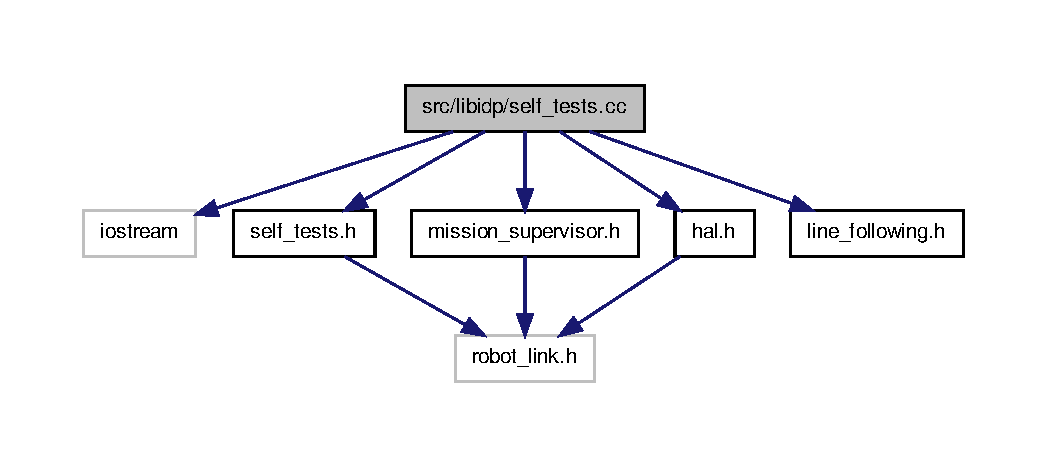
\includegraphics[width=400pt]{self__tests_8cc__incl}
\end{center}
\end{figure}
\subsection*{Namespaces}
\begin{DoxyCompactItemize}
\item 
namespace \hyperlink{namespaceIDP}{IDP}


\begin{DoxyCompactList}\small\item\em Contains all the \hyperlink{namespaceIDP}{IDP} related functionality including libidp and some idpbin classes. \item\end{DoxyCompactList}

\end{DoxyCompactItemize}
\subsection*{Defines}
\begin{DoxyCompactItemize}
\item 
\#define \hyperlink{self__tests_8cc_a14ded244c47bbba850a8a4be6d16c7e3}{MODULE\_\-NAME}~\char`\"{}SelfTests\char`\"{}
\item 
\#define \hyperlink{self__tests_8cc_ae04c5e41f64b51d21bc71565938a59d6}{TRACE\_\-ENABLED}~false
\item 
\#define \hyperlink{self__tests_8cc_a7d2ae674cad5299a52b0e7dceac10087}{DEBUG\_\-ENABLED}~true
\item 
\#define \hyperlink{self__tests_8cc_a580f977f97ee7f7ceb91b1c42306f537}{INFO\_\-ENABLED}~true
\item 
\#define \hyperlink{self__tests_8cc_a292d4ca4e07d63502916a17a853ab606}{ERROR\_\-ENABLED}~true
\end{DoxyCompactItemize}


\subsection{Define Documentation}
\hypertarget{self__tests_8cc_a7d2ae674cad5299a52b0e7dceac10087}{
\index{self\_\-tests.cc@{self\_\-tests.cc}!DEBUG\_\-ENABLED@{DEBUG\_\-ENABLED}}
\index{DEBUG\_\-ENABLED@{DEBUG\_\-ENABLED}!self_tests.cc@{self\_\-tests.cc}}
\subsubsection[{DEBUG\_\-ENABLED}]{\setlength{\rightskip}{0pt plus 5cm}\#define DEBUG\_\-ENABLED~true}}
\label{self__tests_8cc_a7d2ae674cad5299a52b0e7dceac10087}


Definition at line 23 of file self\_\-tests.cc.

\hypertarget{self__tests_8cc_a292d4ca4e07d63502916a17a853ab606}{
\index{self\_\-tests.cc@{self\_\-tests.cc}!ERROR\_\-ENABLED@{ERROR\_\-ENABLED}}
\index{ERROR\_\-ENABLED@{ERROR\_\-ENABLED}!self_tests.cc@{self\_\-tests.cc}}
\subsubsection[{ERROR\_\-ENABLED}]{\setlength{\rightskip}{0pt plus 5cm}\#define ERROR\_\-ENABLED~true}}
\label{self__tests_8cc_a292d4ca4e07d63502916a17a853ab606}


Definition at line 25 of file self\_\-tests.cc.

\hypertarget{self__tests_8cc_a580f977f97ee7f7ceb91b1c42306f537}{
\index{self\_\-tests.cc@{self\_\-tests.cc}!INFO\_\-ENABLED@{INFO\_\-ENABLED}}
\index{INFO\_\-ENABLED@{INFO\_\-ENABLED}!self_tests.cc@{self\_\-tests.cc}}
\subsubsection[{INFO\_\-ENABLED}]{\setlength{\rightskip}{0pt plus 5cm}\#define INFO\_\-ENABLED~true}}
\label{self__tests_8cc_a580f977f97ee7f7ceb91b1c42306f537}


Definition at line 24 of file self\_\-tests.cc.

\hypertarget{self__tests_8cc_a14ded244c47bbba850a8a4be6d16c7e3}{
\index{self\_\-tests.cc@{self\_\-tests.cc}!MODULE\_\-NAME@{MODULE\_\-NAME}}
\index{MODULE\_\-NAME@{MODULE\_\-NAME}!self_tests.cc@{self\_\-tests.cc}}
\subsubsection[{MODULE\_\-NAME}]{\setlength{\rightskip}{0pt plus 5cm}\#define MODULE\_\-NAME~\char`\"{}SelfTests\char`\"{}}}
\label{self__tests_8cc_a14ded244c47bbba850a8a4be6d16c7e3}


Definition at line 21 of file self\_\-tests.cc.

\hypertarget{self__tests_8cc_ae04c5e41f64b51d21bc71565938a59d6}{
\index{self\_\-tests.cc@{self\_\-tests.cc}!TRACE\_\-ENABLED@{TRACE\_\-ENABLED}}
\index{TRACE\_\-ENABLED@{TRACE\_\-ENABLED}!self_tests.cc@{self\_\-tests.cc}}
\subsubsection[{TRACE\_\-ENABLED}]{\setlength{\rightskip}{0pt plus 5cm}\#define TRACE\_\-ENABLED~false}}
\label{self__tests_8cc_ae04c5e41f64b51d21bc71565938a59d6}


Definition at line 22 of file self\_\-tests.cc.


\hypertarget{self__tests_8h}{
\section{libidp/self\_\-tests.h File Reference}
\label{self__tests_8h}\index{libidp/self\_\-tests.h@{libidp/self\_\-tests.h}}
}
{\ttfamily \#include $<$robot\_\-link.h$>$}\par
Include dependency graph for self\_\-tests.h:\nopagebreak
\begin{figure}[H]
\begin{center}
\leavevmode
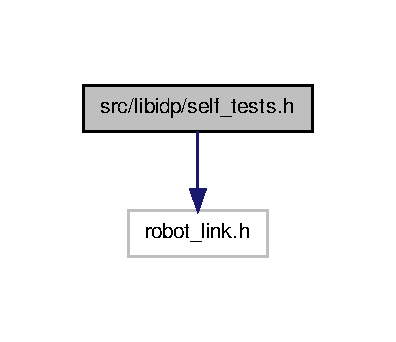
\includegraphics[width=172pt]{self__tests_8h__incl}
\end{center}
\end{figure}
\subsection*{Classes}
\begin{DoxyCompactItemize}
\item 
class \hyperlink{classIDP_1_1SelfTests}{IDP::SelfTests}
\end{DoxyCompactItemize}
\subsection*{Namespaces}
\begin{DoxyCompactItemize}
\item 
namespace \hyperlink{namespaceIDP}{IDP}
\end{DoxyCompactItemize}

\hypertarget{status__watchdog_8cc}{
\section{src/libidp/status\_\-watchdog.cc File Reference}
\label{status__watchdog_8cc}\index{src/libidp/status\_\-watchdog.cc@{src/libidp/status\_\-watchdog.cc}}
}
{\ttfamily \#include \char`\"{}status\_\-watchdog.h\char`\"{}}\par
Include dependency graph for status\_\-watchdog.cc:\nopagebreak
\begin{figure}[H]
\begin{center}
\leavevmode
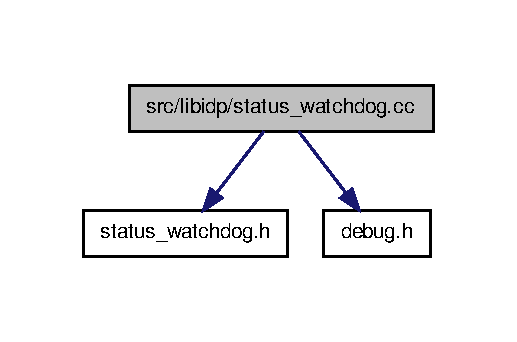
\includegraphics[width=226pt]{status__watchdog_8cc__incl}
\end{center}
\end{figure}
\subsection*{Namespaces}
\begin{DoxyCompactItemize}
\item 
namespace \hyperlink{namespaceIDP}{IDP}
\end{DoxyCompactItemize}

\hypertarget{status__watchdog_8h}{
\section{libidp/status\_\-watchdog.h File Reference}
\label{status__watchdog_8h}\index{libidp/status\_\-watchdog.h@{libidp/status\_\-watchdog.h}}
}
{\ttfamily \#include $<$robot\_\-link.h$>$}\par
Include dependency graph for status\_\-watchdog.h:\nopagebreak
\begin{figure}[H]
\begin{center}
\leavevmode
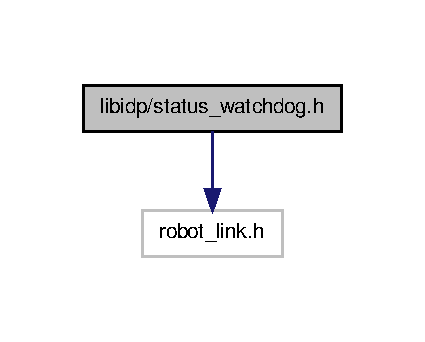
\includegraphics[width=204pt]{status__watchdog_8h__incl}
\end{center}
\end{figure}
This graph shows which files directly or indirectly include this file:\nopagebreak
\begin{figure}[H]
\begin{center}
\leavevmode
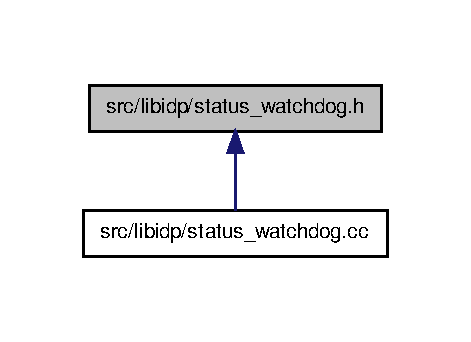
\includegraphics[width=208pt]{status__watchdog_8h__dep__incl}
\end{center}
\end{figure}
\subsection*{Classes}
\begin{DoxyCompactItemize}
\item 
class \hyperlink{classIDP_1_1StatusWatchdog}{IDP::StatusWatchdog}
\begin{DoxyCompactList}\small\item\em Polls the STATUS register of the microcontroller any handles any errors that may arise. \item\end{DoxyCompactList}\end{DoxyCompactItemize}
\subsection*{Namespaces}
\begin{DoxyCompactItemize}
\item 
namespace \hyperlink{namespaceIDP}{IDP}
\end{DoxyCompactItemize}

\printindex
\end{document}
